\PassOptionsToPackage{unicode=true}{hyperref} % options for packages loaded elsewhere
\PassOptionsToPackage{hyphens}{url}
%
\documentclass[ignorenonframetext,]{beamer}
\usepackage{pgfpages}
\setbeamertemplate{caption}[numbered]
\setbeamertemplate{caption label separator}{: }
\setbeamercolor{caption name}{fg=normal text.fg}
\beamertemplatenavigationsymbolsempty
% Prevent slide breaks in the middle of a paragraph:
\widowpenalties 1 10000
\raggedbottom
\setbeamertemplate{part page}{
\centering
\begin{beamercolorbox}[sep=16pt,center]{part title}
  \usebeamerfont{part title}\insertpart\par
\end{beamercolorbox}
}
\setbeamertemplate{section page}{
\centering
\begin{beamercolorbox}[sep=12pt,center]{part title}
  \usebeamerfont{section title}\insertsection\par
\end{beamercolorbox}
}
\setbeamertemplate{subsection page}{
\centering
\begin{beamercolorbox}[sep=8pt,center]{part title}
  \usebeamerfont{subsection title}\insertsubsection\par
\end{beamercolorbox}
}
\AtBeginPart{
  \frame{\partpage}
}
\AtBeginSection{
  \ifbibliography
  \else
    \frame{\sectionpage}
  \fi
}
\AtBeginSubsection{
  \frame{\subsectionpage}
}
\usepackage{lmodern}
\usepackage{amssymb,amsmath}
\usepackage{ifxetex,ifluatex}
\usepackage{fixltx2e} % provides \textsubscript
\ifnum 0\ifxetex 1\fi\ifluatex 1\fi=0 % if pdftex
  \usepackage[T1]{fontenc}
  \usepackage[utf8]{inputenc}
  \usepackage{textcomp} % provides euro and other symbols
\else % if luatex or xelatex
  \usepackage{unicode-math}
  \defaultfontfeatures{Ligatures=TeX,Scale=MatchLowercase}
\fi
% use upquote if available, for straight quotes in verbatim environments
\IfFileExists{upquote.sty}{\usepackage{upquote}}{}
% use microtype if available
\IfFileExists{microtype.sty}{%
\usepackage[]{microtype}
\UseMicrotypeSet[protrusion]{basicmath} % disable protrusion for tt fonts
}{}
\IfFileExists{parskip.sty}{%
\usepackage{parskip}
}{% else
\setlength{\parindent}{0pt}
\setlength{\parskip}{6pt plus 2pt minus 1pt}
}
\usepackage{hyperref}
\hypersetup{
            pdftitle={Lecture 8. Titanic case. Let's kaggle},
            pdfauthor={Олексій Ігнатенко},
            pdfborder={0 0 0},
            breaklinks=true}
\urlstyle{same}  % don't use monospace font for urls
\newif\ifbibliography
\usepackage{color}
\usepackage{fancyvrb}
\newcommand{\VerbBar}{|}
\newcommand{\VERB}{\Verb[commandchars=\\\{\}]}
\DefineVerbatimEnvironment{Highlighting}{Verbatim}{commandchars=\\\{\}}
% Add ',fontsize=\small' for more characters per line
\usepackage{framed}
\definecolor{shadecolor}{RGB}{248,248,248}
\newenvironment{Shaded}{\begin{snugshade}}{\end{snugshade}}
\newcommand{\AlertTok}[1]{\textcolor[rgb]{0.94,0.16,0.16}{#1}}
\newcommand{\AnnotationTok}[1]{\textcolor[rgb]{0.56,0.35,0.01}{\textbf{\textit{#1}}}}
\newcommand{\AttributeTok}[1]{\textcolor[rgb]{0.77,0.63,0.00}{#1}}
\newcommand{\BaseNTok}[1]{\textcolor[rgb]{0.00,0.00,0.81}{#1}}
\newcommand{\BuiltInTok}[1]{#1}
\newcommand{\CharTok}[1]{\textcolor[rgb]{0.31,0.60,0.02}{#1}}
\newcommand{\CommentTok}[1]{\textcolor[rgb]{0.56,0.35,0.01}{\textit{#1}}}
\newcommand{\CommentVarTok}[1]{\textcolor[rgb]{0.56,0.35,0.01}{\textbf{\textit{#1}}}}
\newcommand{\ConstantTok}[1]{\textcolor[rgb]{0.00,0.00,0.00}{#1}}
\newcommand{\ControlFlowTok}[1]{\textcolor[rgb]{0.13,0.29,0.53}{\textbf{#1}}}
\newcommand{\DataTypeTok}[1]{\textcolor[rgb]{0.13,0.29,0.53}{#1}}
\newcommand{\DecValTok}[1]{\textcolor[rgb]{0.00,0.00,0.81}{#1}}
\newcommand{\DocumentationTok}[1]{\textcolor[rgb]{0.56,0.35,0.01}{\textbf{\textit{#1}}}}
\newcommand{\ErrorTok}[1]{\textcolor[rgb]{0.64,0.00,0.00}{\textbf{#1}}}
\newcommand{\ExtensionTok}[1]{#1}
\newcommand{\FloatTok}[1]{\textcolor[rgb]{0.00,0.00,0.81}{#1}}
\newcommand{\FunctionTok}[1]{\textcolor[rgb]{0.00,0.00,0.00}{#1}}
\newcommand{\ImportTok}[1]{#1}
\newcommand{\InformationTok}[1]{\textcolor[rgb]{0.56,0.35,0.01}{\textbf{\textit{#1}}}}
\newcommand{\KeywordTok}[1]{\textcolor[rgb]{0.13,0.29,0.53}{\textbf{#1}}}
\newcommand{\NormalTok}[1]{#1}
\newcommand{\OperatorTok}[1]{\textcolor[rgb]{0.81,0.36,0.00}{\textbf{#1}}}
\newcommand{\OtherTok}[1]{\textcolor[rgb]{0.56,0.35,0.01}{#1}}
\newcommand{\PreprocessorTok}[1]{\textcolor[rgb]{0.56,0.35,0.01}{\textit{#1}}}
\newcommand{\RegionMarkerTok}[1]{#1}
\newcommand{\SpecialCharTok}[1]{\textcolor[rgb]{0.00,0.00,0.00}{#1}}
\newcommand{\SpecialStringTok}[1]{\textcolor[rgb]{0.31,0.60,0.02}{#1}}
\newcommand{\StringTok}[1]{\textcolor[rgb]{0.31,0.60,0.02}{#1}}
\newcommand{\VariableTok}[1]{\textcolor[rgb]{0.00,0.00,0.00}{#1}}
\newcommand{\VerbatimStringTok}[1]{\textcolor[rgb]{0.31,0.60,0.02}{#1}}
\newcommand{\WarningTok}[1]{\textcolor[rgb]{0.56,0.35,0.01}{\textbf{\textit{#1}}}}
\usepackage{graphicx,grffile}
\makeatletter
\def\maxwidth{\ifdim\Gin@nat@width>\linewidth\linewidth\else\Gin@nat@width\fi}
\def\maxheight{\ifdim\Gin@nat@height>\textheight\textheight\else\Gin@nat@height\fi}
\makeatother
% Scale images if necessary, so that they will not overflow the page
% margins by default, and it is still possible to overwrite the defaults
% using explicit options in \includegraphics[width, height, ...]{}
\setkeys{Gin}{width=\maxwidth,height=\maxheight,keepaspectratio}
\setlength{\emergencystretch}{3em}  % prevent overfull lines
\providecommand{\tightlist}{%
  \setlength{\itemsep}{0pt}\setlength{\parskip}{0pt}}
\setcounter{secnumdepth}{0}

% set default figure placement to htbp
\makeatletter
\def\fps@figure{htbp}
\makeatother


\title{Lecture 8. Titanic case. Let's kaggle}
\author{Олексій Ігнатенко}
\date{November 3, 2019}

\begin{document}
\frame{\titlepage}

\begin{frame}[fragile]{Titanic dataset і його аналіз}
\protect\hypertarget{titanic-dataset-ux456-ux439ux43eux433ux43e-ux430ux43dux430ux43bux456ux437}{}

Завантажимо датасет

\begin{Shaded}
\begin{Highlighting}[]
\NormalTok{train <-}\StringTok{ }\KeywordTok{read.csv}\NormalTok{(}\StringTok{"Titanic/train.csv"}\NormalTok{, }\DataTypeTok{stringsAsFactors =} \OtherTok{FALSE}\NormalTok{)}
\NormalTok{test <-}\StringTok{ }\KeywordTok{read.csv}\NormalTok{(}\StringTok{"Titanic/test.csv"}\NormalTok{, }\DataTypeTok{stringsAsFactors =} \OtherTok{FALSE}\NormalTok{)}
\end{Highlighting}
\end{Shaded}

\end{frame}

\begin{frame}[fragile]{Дані, що вони показують}
\protect\hypertarget{ux434ux430ux43dux456-ux449ux43e-ux432ux43eux43dux438-ux43fux43eux43aux430ux437ux443ux44eux442ux44c}{}

\begin{Shaded}
\begin{Highlighting}[]
\KeywordTok{str}\NormalTok{(train)}
\end{Highlighting}
\end{Shaded}

\begin{verbatim}
## 'data.frame':    891 obs. of  12 variables:
##  $ PassengerId: int  1 2 3 4 5 6 7 8 9 10 ...
##  $ Survived   : int  0 1 1 1 0 0 0 0 1 1 ...
##  $ Pclass     : int  3 1 3 1 3 3 1 3 3 2 ...
##  $ Name       : chr  "Braund, Mr. Owen Harris" "Cumings, Mrs. John Bradley (Florence Briggs Thayer)" "Heikkinen, Miss. Laina" "Futrelle, Mrs. Jacques Heath (Lily May Peel)" ...
##  $ Sex        : chr  "male" "female" "female" "female" ...
##  $ Age        : num  22 38 26 35 35 NA 54 2 27 14 ...
##  $ SibSp      : int  1 1 0 1 0 0 0 3 0 1 ...
##  $ Parch      : int  0 0 0 0 0 0 0 1 2 0 ...
##  $ Ticket     : chr  "A/5 21171" "PC 17599" "STON/O2. 3101282" "113803" ...
##  $ Fare       : num  7.25 71.28 7.92 53.1 8.05 ...
##  $ Cabin      : chr  "" "C85" "" "C123" ...
##  $ Embarked   : chr  "S" "C" "S" "S" ...
\end{verbatim}

\end{frame}

\begin{frame}[fragile]{Отже почнемо}
\protect\hypertarget{ux43eux442ux436ux435-ux43fux43eux447ux43dux435ux43cux43e}{}

Підключимо tidyverse

\begin{Shaded}
\begin{Highlighting}[]
\KeywordTok{library}\NormalTok{(tidyverse)}
\end{Highlighting}
\end{Shaded}

\begin{verbatim}
## -- Attaching packages ----------------------------------------------------------------------------------------- tidyverse 1.2.1 --
\end{verbatim}

\begin{verbatim}
## v tibble  2.1.3     v purrr   0.3.3
## v tidyr   1.0.0     v dplyr   0.8.3
## v readr   1.3.1     v stringr 1.4.0
## v tibble  2.1.3     v forcats 0.4.0
\end{verbatim}

\begin{verbatim}
## -- Conflicts -------------------------------------------------------------------------------------------- tidyverse_conflicts() --
## x dplyr::filter() masks stats::filter()
## x dplyr::lag()    masks stats::lag()
\end{verbatim}

\end{frame}

\begin{frame}[fragile]{Додамо відсутні дані з минулої лекції}
\protect\hypertarget{ux434ux43eux434ux430ux43cux43e-ux432ux456ux434ux441ux443ux442ux43dux456-ux434ux430ux43dux456-ux437-ux43cux438ux43dux443ux43bux43eux457-ux43bux435ux43aux446ux456ux457}{}

\begin{Shaded}
\begin{Highlighting}[]
\NormalTok{train}\OperatorTok{$}\NormalTok{Fare[}\KeywordTok{is.na}\NormalTok{(train}\OperatorTok{$}\NormalTok{Fare)}\OperatorTok{==}\OtherTok{TRUE}\NormalTok{] =}\StringTok{ }\KeywordTok{median}\NormalTok{(}\KeywordTok{filter}\NormalTok{(train, Pclass}\OperatorTok{==}\DecValTok{3} \OperatorTok{&}\StringTok{ }\NormalTok{Embarked}\OperatorTok{==}\StringTok{"S"}\NormalTok{)}\OperatorTok{$}\NormalTok{Fare, }\DataTypeTok{na.rm=}\OtherTok{TRUE}\NormalTok{)}
\NormalTok{train}\OperatorTok{$}\NormalTok{Embarked[train}\OperatorTok{$}\NormalTok{Embarked}\OperatorTok{==}\StringTok{""}\NormalTok{] =}\StringTok{ "C"}
\NormalTok{imputed.age <-}\StringTok{ }\KeywordTok{impute.age}\NormalTok{(train}\OperatorTok{$}\NormalTok{Age,train}\OperatorTok{$}\NormalTok{Pclass)}
\NormalTok{train}\OperatorTok{$}\NormalTok{Age <-}\StringTok{ }\NormalTok{imputed.age}
\KeywordTok{colSums}\NormalTok{(}\KeywordTok{is.na}\NormalTok{(train)}\OperatorTok{|}\NormalTok{train}\OperatorTok{==}\StringTok{''}\NormalTok{)}
\end{Highlighting}
\end{Shaded}

\begin{verbatim}
## PassengerId    Survived      Pclass        Name         Sex         Age 
##           0           0           0           0           0           0 
##       SibSp       Parch      Ticket        Fare       Cabin    Embarked 
##           0           0           0           0         687           0
\end{verbatim}

\end{frame}

\begin{frame}[fragile]{Перше наближення і його точність}
\protect\hypertarget{ux43fux435ux440ux448ux435-ux43dux430ux431ux43bux438ux436ux435ux43dux43dux44f-ux456-ux439ux43eux433ux43e-ux442ux43eux447ux43dux456ux441ux442ux44c}{}

\begin{Shaded}
\begin{Highlighting}[]
\NormalTok{test}\OperatorTok{$}\NormalTok{Survived <-}\StringTok{ }\KeywordTok{rep}\NormalTok{(}\DecValTok{0}\NormalTok{, }\DecValTok{418}\NormalTok{)}
\NormalTok{submit <-}\StringTok{ }\KeywordTok{data.frame}\NormalTok{(}\DataTypeTok{PassengerId =}\NormalTok{ test}\OperatorTok{$}\NormalTok{PassengerId, }\DataTypeTok{Survived =}\NormalTok{ test}\OperatorTok{$}\NormalTok{Survived)}
\KeywordTok{write.csv}\NormalTok{(submit, }\DataTypeTok{file =} \StringTok{"theyallperish.csv"}\NormalTok{, }\DataTypeTok{row.names =} \OtherTok{FALSE}\NormalTok{)}
\end{Highlighting}
\end{Shaded}

\end{frame}

\begin{frame}[fragile]{Перевіримо}
\protect\hypertarget{ux43fux435ux440ux435ux432ux456ux440ux438ux43cux43e}{}

\begin{Shaded}
\begin{Highlighting}[]
\NormalTok{knitr}\OperatorTok{::}\KeywordTok{include_graphics}\NormalTok{(}\StringTok{"Submission1.jpeg"}\NormalTok{)}
\end{Highlighting}
\end{Shaded}

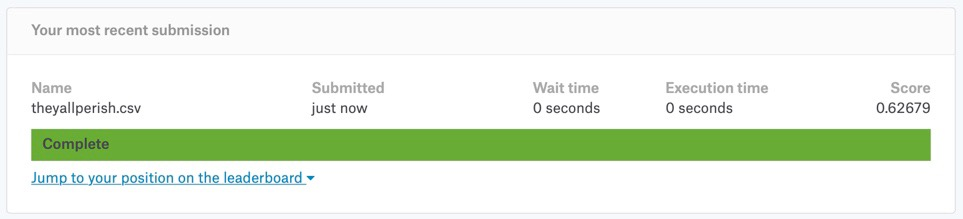
\includegraphics[width=13.38in]{Submission1}

\end{frame}

\begin{frame}[fragile]{Тепер спробуємо покращити результат}
\protect\hypertarget{ux442ux435ux43fux435ux440-ux441ux43fux440ux43eux431ux443ux454ux43cux43e-ux43fux43eux43aux440ux430ux449ux438ux442ux438-ux440ux435ux437ux443ux43bux44cux442ux430ux442}{}

Dplyr + всі жінки врятувались

\begin{Shaded}
\begin{Highlighting}[]
\KeywordTok{library}\NormalTok{(dplyr)}
\NormalTok{female <-}\StringTok{ }\ControlFlowTok{function}\NormalTok{(id)  }\KeywordTok{ifelse}\NormalTok{(test[test}\OperatorTok{$}\NormalTok{PassengerId }\OperatorTok{==}\StringTok{ }\NormalTok{id,]}\OperatorTok{$}\NormalTok{Sex }\OperatorTok{==}\StringTok{ 'female'}\NormalTok{,}\DecValTok{1}\NormalTok{,}\DecValTok{0}\NormalTok{)}

\NormalTok{submit <-}\StringTok{ }\NormalTok{submit }\OperatorTok
\StringTok{  }\KeywordTok{mutate}\NormalTok{(}\DataTypeTok{Survived =} \KeywordTok{female}\NormalTok{(PassengerId)) }
\end{Highlighting}
\end{Shaded}

\end{frame}

\begin{frame}[fragile]{Нова спроба!}
\protect\hypertarget{ux43dux43eux432ux430-ux441ux43fux440ux43eux431ux430}{}

\begin{Shaded}
\begin{Highlighting}[]
\KeywordTok{write.csv}\NormalTok{(submit, }\DataTypeTok{file =} \StringTok{"femalesSurvived.csv"}\NormalTok{, }\DataTypeTok{row.names =} \OtherTok{FALSE}\NormalTok{)}
\end{Highlighting}
\end{Shaded}

\begin{Shaded}
\begin{Highlighting}[]
\NormalTok{knitr}\OperatorTok{::}\KeywordTok{include_graphics}\NormalTok{(}\StringTok{"Submission2.png"}\NormalTok{)}
\end{Highlighting}
\end{Shaded}

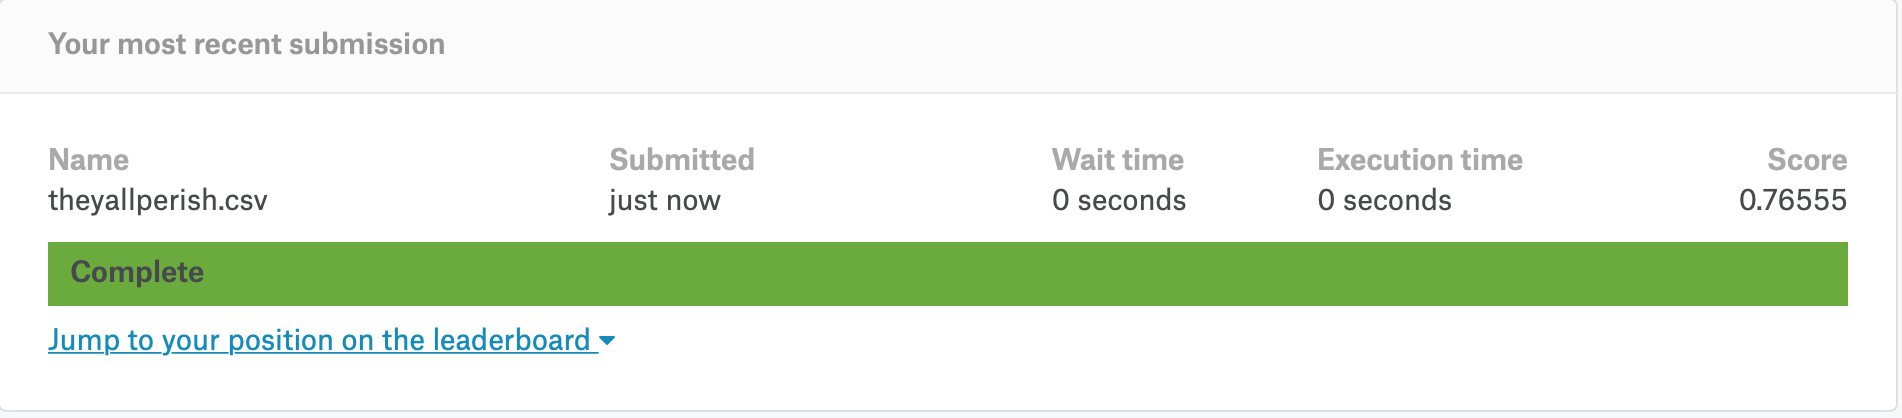
\includegraphics[width=26.42in]{Submission2}

\end{frame}

\begin{frame}[fragile]{Додамо дітей в модель, їх виживання теж вище}
\protect\hypertarget{ux434ux43eux434ux430ux43cux43e-ux434ux456ux442ux435ux439-ux432-ux43cux43eux434ux435ux43bux44c-ux457ux445-ux432ux438ux436ux438ux432ux430ux43dux43dux44f-ux442ux435ux436-ux432ux438ux449ux435}{}

\begin{Shaded}
\begin{Highlighting}[]
\NormalTok{train}\OperatorTok{$}\NormalTok{Child <-}\StringTok{ }\DecValTok{0}
\NormalTok{train}\OperatorTok{$}\NormalTok{Child[train}\OperatorTok{$}\NormalTok{Age }\OperatorTok{<}\StringTok{ }\DecValTok{18}\NormalTok{] <-}\StringTok{ }\DecValTok{1}
\end{Highlighting}
\end{Shaded}

\end{frame}

\begin{frame}[fragile]{Тепер проаналізуємо виживання}
\protect\hypertarget{ux442ux435ux43fux435ux440-ux43fux440ux43eux430ux43dux430ux43bux456ux437ux443ux454ux43cux43e-ux432ux438ux436ux438ux432ux430ux43dux43dux44f}{}

\begin{Shaded}
\begin{Highlighting}[]
\NormalTok{train }\OperatorTok
\StringTok{  }\KeywordTok{group_by}\NormalTok{(Child,Sex) }\OperatorTok
\StringTok{  }\KeywordTok{summarise}\NormalTok{(}\DataTypeTok{survived_number =} \KeywordTok{sum}\NormalTok{(}\KeywordTok{as.numeric}\NormalTok{(Survived) }\OperatorTok{-}\StringTok{ }\DecValTok{1}\NormalTok{),}
            \DataTypeTok{total =} \KeywordTok{n}\NormalTok{())}
\end{Highlighting}
\end{Shaded}

\begin{verbatim}
## # A tibble: 4 x 4
## # Groups:   Child [2]
##   Child Sex    survived_number total
##   <dbl> <chr>            <dbl> <int>
## 1     0 female             -64   259
## 2     0 male              -433   519
## 3     1 female             -17    55
## 4     1 male               -35    58
\end{verbatim}

\end{frame}

\begin{frame}[fragile]{Додамо відсоток}
\protect\hypertarget{ux434ux43eux434ux430ux43cux43e-ux432ux456ux434ux441ux43eux442ux43eux43a}{}

\begin{Shaded}
\begin{Highlighting}[]
\NormalTok{train }\OperatorTok
\StringTok{  }\KeywordTok{group_by}\NormalTok{(Child,Sex) }\OperatorTok
\StringTok{  }\KeywordTok{summarise}\NormalTok{(}\DataTypeTok{survived_number =} \KeywordTok{sum}\NormalTok{(}\KeywordTok{as.numeric}\NormalTok{(Survived) }\OperatorTok{-}\StringTok{ }\DecValTok{1}\NormalTok{),}
            \DataTypeTok{total =} \KeywordTok{n}\NormalTok{(),}
            \DataTypeTok{percent_survived =}\NormalTok{ survived_number }\OperatorTok{/}\StringTok{ }\NormalTok{total)}
\end{Highlighting}
\end{Shaded}

\begin{verbatim}
## # A tibble: 4 x 5
## # Groups:   Child [2]
##   Child Sex    survived_number total percent_survived
##   <dbl> <chr>            <dbl> <int>            <dbl>
## 1     0 female             -64   259           -0.247
## 2     0 male              -433   519           -0.834
## 3     1 female             -17    55           -0.309
## 4     1 male               -35    58           -0.603
\end{verbatim}

\end{frame}

\begin{frame}[fragile]{Тепер додамо клас}
\protect\hypertarget{ux442ux435ux43fux435ux440-ux434ux43eux434ux430ux43cux43e-ux43aux43bux430ux441}{}

\begin{Shaded}
\begin{Highlighting}[]
\NormalTok{train }\OperatorTok
\StringTok{  }\KeywordTok{group_by}\NormalTok{(Child,Sex,Pclass) }\OperatorTok
\StringTok{  }\KeywordTok{summarise}\NormalTok{(}\DataTypeTok{survived_number =} \KeywordTok{sum}\NormalTok{(}\KeywordTok{as.numeric}\NormalTok{(Survived) }\OperatorTok{-}\StringTok{ }\DecValTok{1}\NormalTok{),}
            \DataTypeTok{total =} \KeywordTok{n}\NormalTok{(),}
            \DataTypeTok{percent_survived =}\NormalTok{ survived_number }\OperatorTok{/}\StringTok{ }\NormalTok{total) }\OperatorTok
\StringTok{  }\KeywordTok{arrange}\NormalTok{(}\KeywordTok{desc}\NormalTok{(percent_survived))}
\end{Highlighting}
\end{Shaded}

\begin{verbatim}
## # A tibble: 12 x 6
## # Groups:   Child, Sex [4]
##    Child Sex    Pclass survived_number total percent_survived
##    <dbl> <chr>   <int>           <dbl> <int>            <dbl>
##  1     1 female      2               0    12           0     
##  2     1 male        1               0     4           0     
##  3     0 female      1              -2    86          -0.0233
##  4     0 female      2              -6    64          -0.0938
##  5     1 female      1              -1     8          -0.125 
##  6     1 male        2              -2    11          -0.182 
##  7     1 female      3             -16    35          -0.457 
##  8     0 female      3             -56   109          -0.514 
##  9     0 male        1             -77   118          -0.653 
## 10     1 male        3             -33    43          -0.767 
## 11     0 male        3            -267   304          -0.878 
## 12     0 male        2             -89    97          -0.918
\end{verbatim}

\end{frame}

\begin{frame}[fragile]{Давайте побудуємо на цьому модель}
\protect\hypertarget{ux434ux430ux432ux430ux439ux442ux435-ux43fux43eux431ux443ux434ux443ux454ux43cux43e-ux43dux430-ux446ux44cux43eux43cux443-ux43cux43eux434ux435ux43bux44c}{}

\begin{Shaded}
\begin{Highlighting}[]
\NormalTok{test}\OperatorTok{$}\NormalTok{Survived <-}\StringTok{ }\DecValTok{0}
\NormalTok{test}\OperatorTok{$}\NormalTok{Child <-}\StringTok{ }\DecValTok{0}
\NormalTok{test}\OperatorTok{$}\NormalTok{Child[test}\OperatorTok{$}\NormalTok{Age }\OperatorTok{<}\StringTok{ }\DecValTok{18}\NormalTok{] <-}\StringTok{ }\DecValTok{1}
\NormalTok{test}\OperatorTok{$}\NormalTok{Survived[test}\OperatorTok{$}\NormalTok{Child }\OperatorTok{==}\StringTok{ }\DecValTok{1} \OperatorTok{&}\StringTok{ }\NormalTok{test}\OperatorTok{$}\NormalTok{Pclass }\OperatorTok\StringTok{ }\KeywordTok{c}\NormalTok{(}\DecValTok{1}\NormalTok{,}\DecValTok{2}\NormalTok{)] <-}\StringTok{ }\DecValTok{1}
\NormalTok{test}\OperatorTok{$}\NormalTok{Survived[test}\OperatorTok{$}\NormalTok{Sex }\OperatorTok{==}\StringTok{ 'female'}\NormalTok{] <-}\StringTok{ }\DecValTok{1}
\NormalTok{submit}\OperatorTok{$}\NormalTok{Survived <-}\StringTok{ }\NormalTok{test}\OperatorTok{$}\NormalTok{Survived}
\KeywordTok{write.csv}\NormalTok{(submit, }\DataTypeTok{file =} \StringTok{"impovedSurvived.csv"}\NormalTok{, }\DataTypeTok{row.names =} \OtherTok{FALSE}\NormalTok{)}
\end{Highlighting}
\end{Shaded}

\end{frame}

\begin{frame}[fragile]{Результат}
\protect\hypertarget{ux440ux435ux437ux443ux43bux44cux442ux430ux442}{}

\begin{Shaded}
\begin{Highlighting}[]
\NormalTok{knitr}\OperatorTok{::}\KeywordTok{include_graphics}\NormalTok{(}\StringTok{"Submission3.png"}\NormalTok{)}
\end{Highlighting}
\end{Shaded}

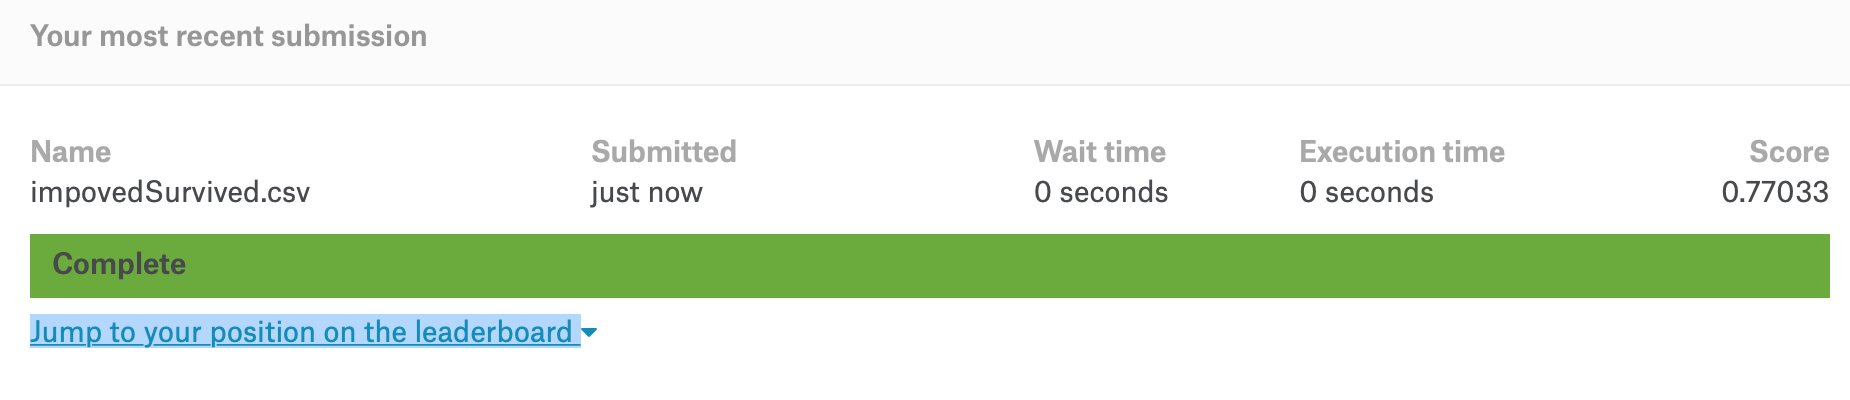
\includegraphics[width=25.69in]{Submission3}

\end{frame}

\begin{frame}[fragile]{Тепер додамо вартість каюти}
\protect\hypertarget{ux442ux435ux43fux435ux440-ux434ux43eux434ux430ux43cux43e-ux432ux430ux440ux442ux456ux441ux442ux44c-ux43aux430ux44eux442ux438}{}

\begin{Shaded}
\begin{Highlighting}[]
\NormalTok{train}\OperatorTok{$}\NormalTok{Fare2 <-}\StringTok{ '30+'}
\NormalTok{train}\OperatorTok{$}\NormalTok{Fare2[train}\OperatorTok{$}\NormalTok{Fare }\OperatorTok{<}\StringTok{ }\DecValTok{30} \OperatorTok{&}\StringTok{ }\NormalTok{train}\OperatorTok{$}\NormalTok{Fare }\OperatorTok{>=}\StringTok{ }\DecValTok{20}\NormalTok{] <-}\StringTok{ '20-30'}
\NormalTok{train}\OperatorTok{$}\NormalTok{Fare2[train}\OperatorTok{$}\NormalTok{Fare }\OperatorTok{<}\StringTok{ }\DecValTok{20} \OperatorTok{&}\StringTok{ }\NormalTok{train}\OperatorTok{$}\NormalTok{Fare }\OperatorTok{>=}\StringTok{ }\DecValTok{10}\NormalTok{] <-}\StringTok{ '10-20'}
\NormalTok{train}\OperatorTok{$}\NormalTok{Fare2[train}\OperatorTok{$}\NormalTok{Fare }\OperatorTok{<}\StringTok{ }\DecValTok{10}\NormalTok{] <-}\StringTok{ '<10'}

\NormalTok{train }\OperatorTok
\StringTok{  }\KeywordTok{group_by}\NormalTok{(Child,Sex,Pclass,Fare2) }\OperatorTok
\StringTok{  }\KeywordTok{summarise}\NormalTok{(}\DataTypeTok{survived_number =} \KeywordTok{sum}\NormalTok{(}\KeywordTok{as.numeric}\NormalTok{(Survived) }\OperatorTok{-}\StringTok{ }\DecValTok{1}\NormalTok{),}
            \DataTypeTok{total =} \KeywordTok{n}\NormalTok{(),}
            \DataTypeTok{percent_survived =}\NormalTok{ survived_number }\OperatorTok{/}\StringTok{ }\NormalTok{total) }\OperatorTok
\StringTok{  }\KeywordTok{arrange}\NormalTok{(}\KeywordTok{desc}\NormalTok{(percent_survived))}
\end{Highlighting}
\end{Shaded}

\begin{verbatim}
## # A tibble: 36 x 7
## # Groups:   Child, Sex, Pclass [12]
##    Child Sex    Pclass Fare2 survived_number total percent_survived
##    <dbl> <chr>   <int> <chr>           <dbl> <int>            <dbl>
##  1     0 female      2 30+                 0     7           0     
##  2     1 female      2 10-20               0     3           0     
##  3     1 female      2 20-30               0     5           0     
##  4     1 female      2 30+                 0     4           0     
##  5     1 male        1 30+                 0     4           0     
##  6     1 male        2 30+                 0     3           0     
##  7     0 female      1 30+                -1    80          -0.0125
##  8     0 female      2 10-20              -3    32          -0.0938
##  9     0 female      2 20-30              -3    25          -0.12  
## 10     1 female      1 30+                -1     8          -0.125 
## # ... with 26 more rows
\end{verbatim}

\end{frame}

\begin{frame}[fragile]{Про які фішки ми забули?}
\protect\hypertarget{ux43fux440ux43e-ux44fux43aux456-ux444ux456ux448ux43aux438-ux43cux438-ux437ux430ux431ux443ux43bux438}{}

\begin{Shaded}
\begin{Highlighting}[]
\NormalTok{train }\OperatorTok
\StringTok{  }\KeywordTok{group_by}\NormalTok{(FamilySize, Title,Pclass,Fare2) }\OperatorTok
\StringTok{  }\KeywordTok{summarise}\NormalTok{(}\DataTypeTok{percent_survived =} \KeywordTok{sum}\NormalTok{(}\KeywordTok{as.numeric}\NormalTok{(Survived) }\OperatorTok{-}\StringTok{ }\DecValTok{1}\NormalTok{) }\OperatorTok{/}\StringTok{ }\KeywordTok{n}\NormalTok{()) }\OperatorTok
\StringTok{  }\KeywordTok{arrange}\NormalTok{(}\KeywordTok{desc}\NormalTok{(percent_survived))}
\end{Highlighting}
\end{Shaded}

\begin{verbatim}
## # A tibble: 135 x 5
## # Groups:   FamilySize, Title, Pclass [78]
##    FamilySize Title Pclass Fare2 percent_survived
##         <dbl> <chr>  <int> <chr>            <dbl>
##  1          1 Col        1 30+                  0
##  2          1 Dr         1 20-30                0
##  3          1 Lady       1 30+                  0
##  4          1 Miss       1 30+                  0
##  5          1 Miss       2 20-30                0
##  6          1 Miss       2 30+                  0
##  7          1 Mrs        1 20-30                0
##  8          1 Mrs        1 30+                  0
##  9          1 Sir        1 30+                  0
## 10          2 Lady       1 30+                  0
## # ... with 125 more rows
\end{verbatim}

\end{frame}

\begin{frame}[fragile]{Ще одна штука}
\protect\hypertarget{ux449ux435-ux43eux434ux43dux430-ux448ux442ux443ux43aux430}{}

\begin{Shaded}
\begin{Highlighting}[]
\KeywordTok{colSums}\NormalTok{(}\KeywordTok{is.na}\NormalTok{(test)}\OperatorTok{|}\NormalTok{test}\OperatorTok{==}\StringTok{''}\NormalTok{)}
\end{Highlighting}
\end{Shaded}

\begin{verbatim}
## PassengerId      Pclass        Name         Sex         Age       SibSp 
##           0           0           0           0          86           0 
##       Parch      Ticket        Fare       Cabin    Embarked    Survived 
##           0           0           1         327           0           0 
##       Child 
##           0
\end{verbatim}

Потрібно внести дані!

\end{frame}

\begin{frame}[fragile]{Внесення пропущених даних}
\protect\hypertarget{ux432ux43dux435ux441ux435ux43dux43dux44f-ux43fux440ux43eux43fux443ux449ux435ux43dux438ux445-ux434ux430ux43dux438ux445}{}

\begin{Shaded}
\begin{Highlighting}[]
\NormalTok{imputed.age <-}\StringTok{ }\KeywordTok{impute.age}\NormalTok{(test}\OperatorTok{$}\NormalTok{Age,test}\OperatorTok{$}\NormalTok{Pclass)}
\NormalTok{test}\OperatorTok{$}\NormalTok{Age <-}\StringTok{ }\NormalTok{imputed.age}
\KeywordTok{colSums}\NormalTok{(}\KeywordTok{is.na}\NormalTok{(test)}\OperatorTok{|}\NormalTok{test}\OperatorTok{==}\StringTok{''}\NormalTok{)}
\end{Highlighting}
\end{Shaded}

\begin{verbatim}
## PassengerId      Pclass        Name         Sex         Age       SibSp 
##           0           0           0           0           0           0 
##       Parch      Ticket        Fare       Cabin    Embarked    Survived 
##           0           0           1         327           0           0 
##       Child 
##           0
\end{verbatim}

\end{frame}

\begin{frame}[fragile]{Що з чеком}
\protect\hypertarget{ux449ux43e-ux437-ux447ux435ux43aux43eux43c}{}

\begin{Shaded}
\begin{Highlighting}[]
\NormalTok{test[}\KeywordTok{is.na}\NormalTok{(test}\OperatorTok{$}\NormalTok{Fare),]}
\end{Highlighting}
\end{Shaded}

\begin{verbatim}
##     PassengerId Pclass               Name  Sex  Age SibSp Parch Ticket Fare
## 153        1044      3 Storey, Mr. Thomas male 60.5     0     0   3701   NA
##     Cabin Embarked Survived Child
## 153              S        0     0
\end{verbatim}

\begin{Shaded}
\begin{Highlighting}[]
\NormalTok{test}\OperatorTok{$}\NormalTok{Fare[}\KeywordTok{is.na}\NormalTok{(test}\OperatorTok{$}\NormalTok{Fare)}\OperatorTok{==}\OtherTok{TRUE}\NormalTok{] =}\StringTok{ }\KeywordTok{median}\NormalTok{(}\KeywordTok{filter}\NormalTok{(test, Pclass}\OperatorTok{==}\DecValTok{3} \OperatorTok{&}\StringTok{ }\NormalTok{Embarked}\OperatorTok{==}\StringTok{"S"}\NormalTok{)}\OperatorTok{$}\NormalTok{Fare, }\DataTypeTok{na.rm=}\OtherTok{TRUE}\NormalTok{)}
\end{Highlighting}
\end{Shaded}

\end{frame}

\begin{frame}[fragile]{Занесемо наші результати для}
\protect\hypertarget{ux437ux430ux43dux435ux441ux435ux43cux43e-ux43dux430ux448ux456-ux440ux435ux437ux443ux43bux44cux442ux430ux442ux438-ux434ux43bux44f}{}

\begin{Shaded}
\begin{Highlighting}[]
\NormalTok{test}\OperatorTok{$}\NormalTok{Survived <-}\StringTok{ }\DecValTok{0}
\NormalTok{test}\OperatorTok{$}\NormalTok{Child[test}\OperatorTok{$}\NormalTok{Age }\OperatorTok{<}\StringTok{ }\DecValTok{18}\NormalTok{] <-}\StringTok{ }\DecValTok{1}
\NormalTok{test}\OperatorTok{$}\NormalTok{Survived[test}\OperatorTok{$}\NormalTok{Child }\OperatorTok{==}\StringTok{ }\DecValTok{1} \OperatorTok{&}\StringTok{ }\NormalTok{test}\OperatorTok{$}\NormalTok{Pclass }\OperatorTok\StringTok{ }\KeywordTok{c}\NormalTok{(}\DecValTok{1}\NormalTok{,}\DecValTok{2}\NormalTok{)] <-}\StringTok{ }\DecValTok{1}
\NormalTok{test}\OperatorTok{$}\NormalTok{Survived[test}\OperatorTok{$}\NormalTok{Sex }\OperatorTok{==}\StringTok{ 'female'}\NormalTok{] <-}\StringTok{ }\DecValTok{1}
\NormalTok{test}\OperatorTok{$}\NormalTok{Survived[test}\OperatorTok{$}\NormalTok{Sex }\OperatorTok{==}\StringTok{ 'female'} \OperatorTok{&}\StringTok{ }\NormalTok{test}\OperatorTok{$}\NormalTok{Pclass }\OperatorTok{==}\StringTok{ }\DecValTok{3} \OperatorTok{&}\StringTok{ }\NormalTok{test}\OperatorTok{$}\NormalTok{Fare }\OperatorTok{>=}\StringTok{ }\DecValTok{20}\NormalTok{] <-}\StringTok{ }\DecValTok{0}
\NormalTok{submit}\OperatorTok{$}\NormalTok{Survived <-}\StringTok{ }\NormalTok{test}\OperatorTok{$}\NormalTok{Survived}
\KeywordTok{write.csv}\NormalTok{(submit, }\DataTypeTok{file =} \StringTok{"impovedSurvived.csv"}\NormalTok{, }\DataTypeTok{row.names =} \OtherTok{FALSE}\NormalTok{)}
\end{Highlighting}
\end{Shaded}

\end{frame}

\begin{frame}[fragile]{Результат}
\protect\hypertarget{ux440ux435ux437ux443ux43bux44cux442ux430ux442-1}{}

\begin{Shaded}
\begin{Highlighting}[]
\NormalTok{knitr}\OperatorTok{::}\KeywordTok{include_graphics}\NormalTok{(}\StringTok{"Submission4.png"}\NormalTok{)}
\end{Highlighting}
\end{Shaded}


\includegraphics[width=26.36in]{Submission4}

\end{frame}

\begin{frame}[fragile]{Дерева рішень}
\protect\hypertarget{ux434ux435ux440ux435ux432ux430-ux440ux456ux448ux435ux43dux44c}{}

\begin{Shaded}
\begin{Highlighting}[]
\KeywordTok{library}\NormalTok{(rpart)}
\NormalTok{fit <-}\StringTok{ }\KeywordTok{rpart}\NormalTok{(Survived }\OperatorTok{~}\StringTok{ }\NormalTok{Pclass }\OperatorTok{+}\StringTok{ }\NormalTok{Sex }\OperatorTok{+}\StringTok{ }\NormalTok{Age }\OperatorTok{+}\StringTok{ }\NormalTok{SibSp }\OperatorTok{+}\StringTok{ }\NormalTok{Parch }\OperatorTok{+}\StringTok{ }\NormalTok{Fare }\OperatorTok{+}\StringTok{ }\NormalTok{Embarked,}
               \DataTypeTok{data=}\NormalTok{train,}
               \DataTypeTok{method=}\StringTok{"class"}\NormalTok{)}
\end{Highlighting}
\end{Shaded}

\end{frame}

\begin{frame}[fragile]{Візуалізація}
\protect\hypertarget{ux432ux456ux437ux443ux430ux43bux456ux437ux430ux446ux456ux44f}{}

\begin{Shaded}
\begin{Highlighting}[]
\KeywordTok{plot}\NormalTok{(fit)}
\KeywordTok{text}\NormalTok{(fit)}
\end{Highlighting}
\end{Shaded}

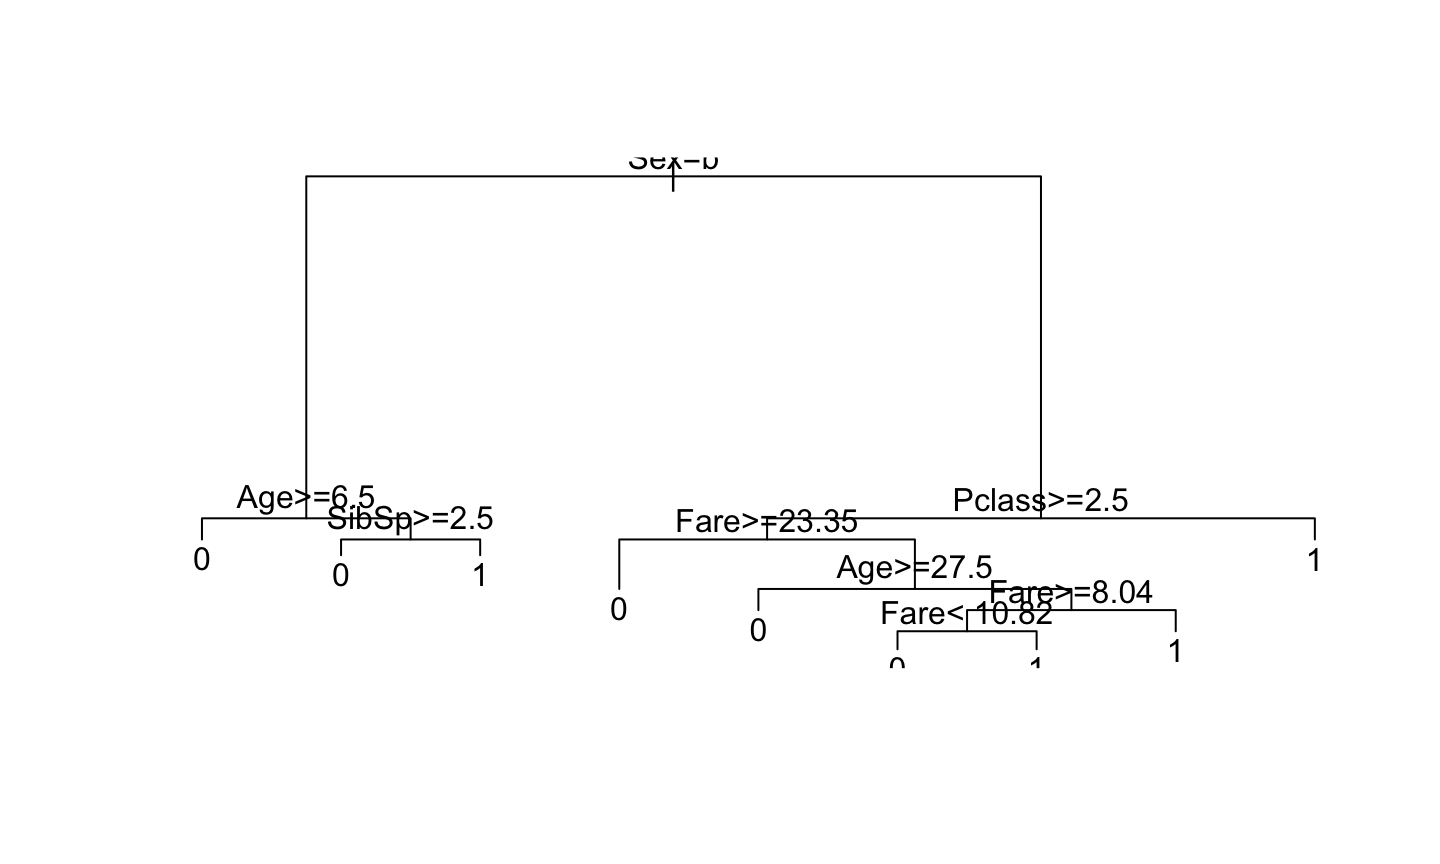
\includegraphics{Lecture8_files/figure-beamer/unnamed-chunk-26-1.pdf}
\#\# Але є добрі люди

\begin{Shaded}
\begin{Highlighting}[]
\KeywordTok{library}\NormalTok{(rattle)}
\end{Highlighting}
\end{Shaded}

\begin{verbatim}
## Rattle: A free graphical interface for data science with R.
## Version 5.2.0 Copyright (c) 2006-2018 Togaware Pty Ltd.
## Type 'rattle()' to shake, rattle, and roll your data.
\end{verbatim}

\begin{Shaded}
\begin{Highlighting}[]
\KeywordTok{library}\NormalTok{(rpart.plot)}
\KeywordTok{library}\NormalTok{(RColorBrewer)}
\end{Highlighting}
\end{Shaded}

\end{frame}

\begin{frame}[fragile]{Тепер візуалізація буде краще}
\protect\hypertarget{ux442ux435ux43fux435ux440-ux432ux456ux437ux443ux430ux43bux456ux437ux430ux446ux456ux44f-ux431ux443ux434ux435-ux43aux440ux430ux449ux435}{}

\begin{Shaded}
\begin{Highlighting}[]
\KeywordTok{fancyRpartPlot}\NormalTok{(fit)}
\end{Highlighting}
\end{Shaded}

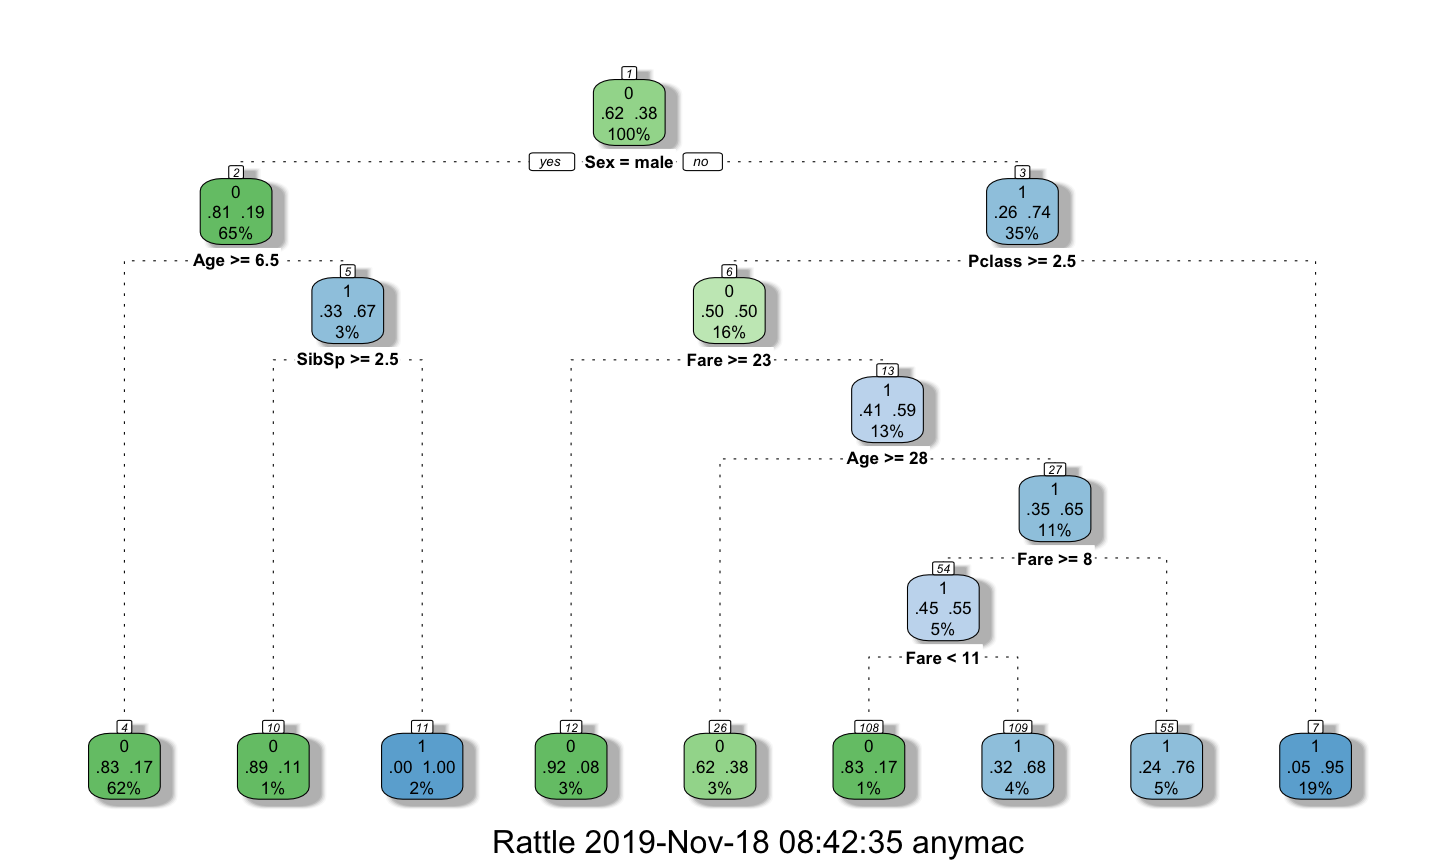
\includegraphics{Lecture8_files/figure-beamer/unnamed-chunk-28-1.pdf}

\end{frame}

\begin{frame}[fragile]{Як робити прогноз на основі дерева?}
\protect\hypertarget{ux44fux43a-ux440ux43eux431ux438ux442ux438-ux43fux440ux43eux433ux43dux43eux437-ux43dux430-ux43eux441ux43dux43eux432ux456-ux434ux435ux440ux435ux432ux430}{}

\begin{Shaded}
\begin{Highlighting}[]
\NormalTok{Prediction <-}\StringTok{ }\KeywordTok{predict}\NormalTok{(fit, test, }\DataTypeTok{type =} \StringTok{"class"}\NormalTok{)}
\NormalTok{submit <-}\StringTok{ }\KeywordTok{data.frame}\NormalTok{(}\DataTypeTok{PassengerId =}\NormalTok{ test}\OperatorTok{$}\NormalTok{PassengerId, }\DataTypeTok{Survived =}\NormalTok{ Prediction)}
\KeywordTok{write.csv}\NormalTok{(submit, }\DataTypeTok{file =} \StringTok{"myfirstdtree.csv"}\NormalTok{, }\DataTypeTok{row.names =} \OtherTok{FALSE}\NormalTok{)}
\end{Highlighting}
\end{Shaded}

\end{frame}

\begin{frame}[fragile]{Ще одна спроба}
\protect\hypertarget{ux449ux435-ux43eux434ux43dux430-ux441ux43fux440ux43eux431ux430}{}

\begin{Shaded}
\begin{Highlighting}[]
\NormalTok{fit <-}\StringTok{ }\KeywordTok{rpart}\NormalTok{(Survived }\OperatorTok{~}\StringTok{ }\NormalTok{Pclass }\OperatorTok{+}\StringTok{ }\NormalTok{Sex }\OperatorTok{+}\StringTok{ }\NormalTok{Age }\OperatorTok{+}\StringTok{ }\NormalTok{Fare2 }\OperatorTok{+}\StringTok{ }\NormalTok{Child }\OperatorTok{+}\StringTok{ }\NormalTok{SibSp }\OperatorTok{+}\StringTok{ }\NormalTok{Parch,}
               \DataTypeTok{data=}\NormalTok{train,}
               \DataTypeTok{method=}\StringTok{"class"}\NormalTok{)}
\KeywordTok{fancyRpartPlot}\NormalTok{(fit)}
\end{Highlighting}
\end{Shaded}

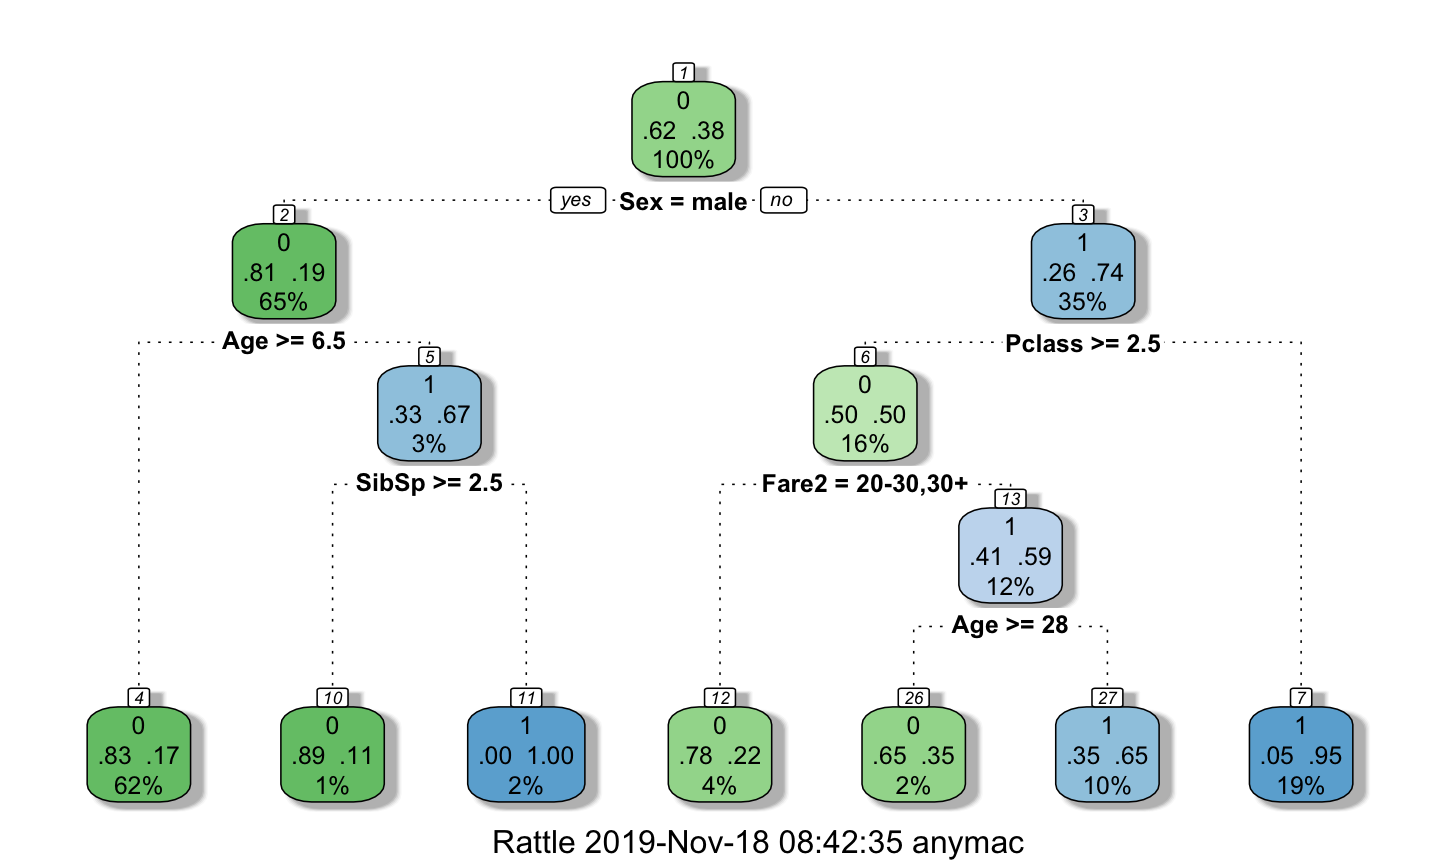
\includegraphics{Lecture8_files/figure-beamer/unnamed-chunk-30-1.pdf}

\end{frame}

\begin{frame}[fragile]{Інженерія особливостей (Feature engineering)}
\protect\hypertarget{ux456ux43dux436ux435ux43dux435ux440ux456ux44f-ux43eux441ux43eux431ux43bux438ux432ux43eux441ux442ux435ux439-feature-engineering}{}

Було б непогано виділити звернення? Можливо незаміжніх рятують краще за
інших. А жінок рятують краще за чоловіків?

\begin{Shaded}
\begin{Highlighting}[]
\NormalTok{train}\OperatorTok{$}\NormalTok{Title <-}\StringTok{ }\KeywordTok{gsub}\NormalTok{(}\StringTok{"^.*, (.*?)}\CharTok{\textbackslash{}\textbackslash{}}\StringTok{..*$"}\NormalTok{, }\StringTok{"}\CharTok{\textbackslash{}\textbackslash{}}\StringTok{1"}\NormalTok{, train}\OperatorTok{$}\NormalTok{Name)}
\KeywordTok{table}\NormalTok{(train}\OperatorTok{$}\NormalTok{Sex, train}\OperatorTok{$}\NormalTok{Title)}
\end{Highlighting}
\end{Shaded}

\begin{verbatim}
##         
##          Capt Col Don  Dr Jonkheer Lady Major Master Miss Mlle Mme  Mr Mrs  Ms
##   female    0   0   0   1        0    1     0      0  182    2   1   0 125   1
##   male      1   2   1   6        1    0     2     40    0    0   0 517   0   0
##         
##          Rev Sir the Countess
##   female   0   0            1
##   male     6   1            0
\end{verbatim}

але їх тут дуже багато

\end{frame}

\begin{frame}[fragile]{Зменшимо кількість}
\protect\hypertarget{ux437ux43cux435ux43dux448ux438ux43cux43e-ux43aux456ux43bux44cux43aux456ux441ux442ux44c}{}

\begin{Shaded}
\begin{Highlighting}[]
\NormalTok{train}\OperatorTok{$}\NormalTok{Title[train}\OperatorTok{$}\NormalTok{Title }\OperatorTok{==}\StringTok{ 'Mlle'} \OperatorTok{|}\StringTok{ }\NormalTok{train}\OperatorTok{$}\NormalTok{Title }\OperatorTok{==}\StringTok{ 'Ms'}\NormalTok{] <-}\StringTok{ 'Miss'} 
\NormalTok{train}\OperatorTok{$}\NormalTok{Title[train}\OperatorTok{$}\NormalTok{Title }\OperatorTok{==}\StringTok{ 'Mme'}\NormalTok{]  <-}\StringTok{ 'Mrs'} 
\NormalTok{train}\OperatorTok{$}\NormalTok{Title[train}\OperatorTok{$}\NormalTok{Title }\OperatorTok\StringTok{ }\KeywordTok{c}\NormalTok{(}\StringTok{'Capt'}\NormalTok{, }\StringTok{'Don'}\NormalTok{, }\StringTok{'Major'}\NormalTok{, }\StringTok{'Sir'}\NormalTok{, }\StringTok{'Jonkheer'}\NormalTok{)] <-}\StringTok{ 'Sir'}
\NormalTok{train}\OperatorTok{$}\NormalTok{Title[train}\OperatorTok{$}\NormalTok{Title }\OperatorTok\StringTok{ }\KeywordTok{c}\NormalTok{(}\StringTok{'Dona'}\NormalTok{, }\StringTok{'Lady'}\NormalTok{, }\StringTok{'the Countess'}\NormalTok{)] <-}\StringTok{ 'Lady'}
\KeywordTok{table}\NormalTok{(train}\OperatorTok{$}\NormalTok{Sex, train}\OperatorTok{$}\NormalTok{Title)}
\end{Highlighting}
\end{Shaded}

\begin{verbatim}
##         
##          Col  Dr Lady Master Miss  Mr Mrs Rev Sir
##   female   0   1    2      0  185   0 126   0   0
##   male     2   6    0     40    0 517   0   6   6
\end{verbatim}

\end{frame}

\begin{frame}[fragile]{Розмір сім'ї}
\protect\hypertarget{ux440ux43eux437ux43cux456ux440-ux441ux456ux43cux457}{}

\begin{Shaded}
\begin{Highlighting}[]
\NormalTok{FamilySize <-}\StringTok{ }\NormalTok{train}\OperatorTok{$}\NormalTok{SibSp }\OperatorTok{+}\StringTok{ }\NormalTok{train}\OperatorTok{$}\NormalTok{Parch }\OperatorTok{+}\StringTok{ }\DecValTok{1}

\KeywordTok{table}\NormalTok{(FamilySize)}
\end{Highlighting}
\end{Shaded}

\begin{verbatim}
## FamilySize
##   1   2   3   4   5   6   7   8  11 
## 537 161 102  29  15  22  12   6   7
\end{verbatim}

Знов таки - багато категорій

\end{frame}

\begin{frame}[fragile]{Три типи сім'ї}
\protect\hypertarget{ux442ux440ux438-ux442ux438ux43fux438-ux441ux456ux43cux457}{}

\begin{Shaded}
\begin{Highlighting}[]
\NormalTok{train}\OperatorTok{$}\NormalTok{FamilySize <-}\StringTok{ }\KeywordTok{sapply}\NormalTok{(}\DecValTok{1}\OperatorTok{:}\KeywordTok{nrow}\NormalTok{(train), }\ControlFlowTok{function}\NormalTok{(x) }
                          \KeywordTok{ifelse}\NormalTok{(FamilySize[x]}\OperatorTok{==}\DecValTok{1}\NormalTok{, }\StringTok{"Single"}\NormalTok{, }
                          \KeywordTok{ifelse}\NormalTok{(FamilySize[x]}\OperatorTok{>}\DecValTok{4}\NormalTok{, }\StringTok{"Large"}\NormalTok{, }\StringTok{"Small"}\NormalTok{)))}

\KeywordTok{table}\NormalTok{(train}\OperatorTok{$}\NormalTok{FamilySize)}
\end{Highlighting}
\end{Shaded}

\begin{verbatim}
## 
##  Large Single  Small 
##     62    537    292
\end{verbatim}

\end{frame}

\begin{frame}[fragile]{Аналіз даних}
\protect\hypertarget{ux430ux43dux430ux43bux456ux437-ux434ux430ux43dux438ux445}{}

\begin{Shaded}
\begin{Highlighting}[]
\NormalTok{train}\OperatorTok{$}\NormalTok{Survived =}\StringTok{ }\KeywordTok{factor}\NormalTok{(train}\OperatorTok{$}\NormalTok{Survived)}
\NormalTok{train}\OperatorTok{$}\NormalTok{Pclass =}\StringTok{ }\KeywordTok{factor}\NormalTok{(train}\OperatorTok{$}\NormalTok{Pclass)}
\NormalTok{train}\OperatorTok{$}\NormalTok{Sex =}\StringTok{ }\KeywordTok{factor}\NormalTok{(train}\OperatorTok{$}\NormalTok{Sex)}
\NormalTok{train}\OperatorTok{$}\NormalTok{Embarked =}\StringTok{ }\KeywordTok{factor}\NormalTok{(train}\OperatorTok{$}\NormalTok{Embarked)}
\NormalTok{train}\OperatorTok{$}\NormalTok{Title =}\StringTok{ }\KeywordTok{factor}\NormalTok{(train}\OperatorTok{$}\NormalTok{Title)}
\NormalTok{train}\OperatorTok{$}\NormalTok{FamilySize =}\StringTok{ }\KeywordTok{factor}\NormalTok{(train}\OperatorTok{$}\NormalTok{FamilySize, }\DataTypeTok{levels=}\KeywordTok{c}\NormalTok{(}\StringTok{"Single"}\NormalTok{,}\StringTok{"Small"}\NormalTok{,}\StringTok{"Large"}\NormalTok{))}

\CommentTok{#Checking the structure of the data}
\KeywordTok{str}\NormalTok{(train)}
\end{Highlighting}
\end{Shaded}

\begin{verbatim}
## 'data.frame':    891 obs. of  16 variables:
##  $ PassengerId: int  1 2 3 4 5 6 7 8 9 10 ...
##  $ Survived   : Factor w/ 2 levels "0","1": 1 2 2 2 1 1 1 1 2 2 ...
##  $ Pclass     : Factor w/ 3 levels "1","2","3": 3 1 3 1 3 3 1 3 3 2 ...
##  $ Name       : chr  "Braund, Mr. Owen Harris" "Cumings, Mrs. John Bradley (Florence Briggs Thayer)" "Heikkinen, Miss. Laina" "Futrelle, Mrs. Jacques Heath (Lily May Peel)" ...
##  $ Sex        : Factor w/ 2 levels "female","male": 2 1 1 1 2 2 2 2 1 1 ...
##  $ Age        : num  22 38 26 35 35 25 54 2 27 14 ...
##  $ SibSp      : int  1 1 0 1 0 0 0 3 0 1 ...
##  $ Parch      : int  0 0 0 0 0 0 0 1 2 0 ...
##  $ Ticket     : chr  "A/5 21171" "PC 17599" "STON/O2. 3101282" "113803" ...
##  $ Fare       : num  7.25 71.28 7.92 53.1 8.05 ...
##  $ Cabin      : chr  "" "C85" "" "C123" ...
##  $ Embarked   : Factor w/ 3 levels "C","Q","S": 3 1 3 3 3 2 3 3 3 1 ...
##  $ Child      : num  0 0 0 0 0 0 0 1 0 1 ...
##  $ Fare2      : chr  "<10" "30+" "<10" "30+" ...
##  $ FamilySize : Factor w/ 3 levels "Single","Small",..: 2 2 1 2 1 1 1 3 2 2 ...
##  $ Title      : Factor w/ 9 levels "Col","Dr","Lady",..: 6 7 5 7 6 6 6 4 7 7 ...
\end{verbatim}

\end{frame}

\begin{frame}[fragile]{Отже повне дерево}
\protect\hypertarget{ux43eux442ux436ux435-ux43fux43eux432ux43dux435-ux434ux435ux440ux435ux432ux43e}{}

\begin{Shaded}
\begin{Highlighting}[]
\NormalTok{fit <-}\StringTok{ }\KeywordTok{rpart}\NormalTok{(Survived }\OperatorTok{~}\StringTok{ }\NormalTok{Pclass }\OperatorTok{+}\StringTok{ }\NormalTok{Sex }\OperatorTok{+}\StringTok{ }\NormalTok{Age }\OperatorTok{+}\StringTok{ }\NormalTok{Fare }\OperatorTok{+}\StringTok{ }\NormalTok{Embarked }\OperatorTok{+}\StringTok{ }\NormalTok{Child }\OperatorTok{+}\StringTok{ }\NormalTok{SibSp }\OperatorTok{+}\StringTok{ }\NormalTok{Parch,}
               \DataTypeTok{data=}\NormalTok{train,}
               \DataTypeTok{method=}\StringTok{"class"}\NormalTok{)}
\KeywordTok{fancyRpartPlot}\NormalTok{(fit)}
\end{Highlighting}
\end{Shaded}

\includegraphics{Lecture8_files/figure-beamer/unnamed-chunk-36-1.pdf}

\end{frame}

\begin{frame}[fragile]{Додамо звернення до тесту}
\protect\hypertarget{ux434ux43eux434ux430ux43cux43e-ux437ux432ux435ux440ux43dux435ux43dux43dux44f-ux434ux43e-ux442ux435ux441ux442ux443}{}

\begin{Shaded}
\begin{Highlighting}[]
\NormalTok{test}\OperatorTok{$}\NormalTok{Title <-}\StringTok{ }\KeywordTok{gsub}\NormalTok{(}\StringTok{"^.*, (.*?)}\CharTok{\textbackslash{}\textbackslash{}}\StringTok{..*$"}\NormalTok{, }\StringTok{"}\CharTok{\textbackslash{}\textbackslash{}}\StringTok{1"}\NormalTok{, test}\OperatorTok{$}\NormalTok{Name)}
\NormalTok{test}\OperatorTok{$}\NormalTok{Title[test}\OperatorTok{$}\NormalTok{Title }\OperatorTok{==}\StringTok{ 'Mlle'} \OperatorTok{|}\StringTok{ }\NormalTok{test}\OperatorTok{$}\NormalTok{Title }\OperatorTok{==}\StringTok{ 'Ms'}\NormalTok{] <-}\StringTok{ 'Miss'} 
\NormalTok{test}\OperatorTok{$}\NormalTok{Title[test}\OperatorTok{$}\NormalTok{Title }\OperatorTok{==}\StringTok{ 'Mme'}\NormalTok{]  <-}\StringTok{ 'Mrs'} 
\NormalTok{test}\OperatorTok{$}\NormalTok{Title[test}\OperatorTok{$}\NormalTok{Title }\OperatorTok\StringTok{ }\KeywordTok{c}\NormalTok{(}\StringTok{'Capt'}\NormalTok{, }\StringTok{'Don'}\NormalTok{, }\StringTok{'Major'}\NormalTok{, }\StringTok{'Sir'}\NormalTok{, }\StringTok{'Jonkheer'}\NormalTok{)] <-}\StringTok{ 'Sir'}
\NormalTok{test}\OperatorTok{$}\NormalTok{Title[test}\OperatorTok{$}\NormalTok{Title }\OperatorTok\StringTok{ }\KeywordTok{c}\NormalTok{(}\StringTok{'Dona'}\NormalTok{, }\StringTok{'Lady'}\NormalTok{, }\StringTok{'the Countess'}\NormalTok{)] <-}\StringTok{ 'Lady'}
\KeywordTok{table}\NormalTok{(train}\OperatorTok{$}\NormalTok{Sex, train}\OperatorTok{$}\NormalTok{Title)}
\end{Highlighting}
\end{Shaded}

\begin{verbatim}
##         
##          Col  Dr Lady Master Miss  Mr Mrs Rev Sir
##   female   0   1    2      0  185   0 126   0   0
##   male     2   6    0     40    0 517   0   6   6
\end{verbatim}

\begin{Shaded}
\begin{Highlighting}[]
\KeywordTok{table}\NormalTok{(test}\OperatorTok{$}\NormalTok{Sex, test}\OperatorTok{$}\NormalTok{Title)}
\end{Highlighting}
\end{Shaded}

\begin{verbatim}
##         
##          Col  Dr Lady Master Miss  Mr Mrs Rev
##   female   0   0    1      0   79   0  72   0
##   male     2   1    0     21    0 240   0   2
\end{verbatim}

\end{frame}

\begin{frame}[fragile]{Будуємо дерево}
\protect\hypertarget{ux431ux443ux434ux443ux454ux43cux43e-ux434ux435ux440ux435ux432ux43e}{}

\begin{Shaded}
\begin{Highlighting}[]
\NormalTok{train}\OperatorTok{$}\NormalTok{Pclass <-}\StringTok{ }\KeywordTok{factor}\NormalTok{(train}\OperatorTok{$}\NormalTok{Pclass)}
\NormalTok{test}\OperatorTok{$}\NormalTok{Pclass <-}\StringTok{ }\KeywordTok{factor}\NormalTok{(test}\OperatorTok{$}\NormalTok{Pclass)}
\NormalTok{fit <-}\StringTok{ }\KeywordTok{rpart}\NormalTok{(Survived }\OperatorTok{~}\StringTok{ }\NormalTok{Pclass }\OperatorTok{+}\StringTok{ }\NormalTok{Sex }\OperatorTok{+}\StringTok{ }\NormalTok{Age }\OperatorTok{+}\StringTok{ }\NormalTok{Fare }\OperatorTok{+}\StringTok{ }\NormalTok{Title,}
               \DataTypeTok{data=}\NormalTok{train,}
               \DataTypeTok{method=}\StringTok{"class"}\NormalTok{)}
\KeywordTok{fancyRpartPlot}\NormalTok{(fit)}
\end{Highlighting}
\end{Shaded}

\end{frame}

\begin{frame}{Будуємо дерево}
\protect\hypertarget{ux431ux443ux434ux443ux454ux43cux43e-ux434ux435ux440ux435ux432ux43e-1}{}

\includegraphics{Lecture8_files/figure-beamer/unnamed-chunk-39-1.pdf}

\end{frame}

\begin{frame}[fragile]{Є покращення для дерева, але гірше за нашу просту
модель}
\protect\hypertarget{ux454-ux43fux43eux43aux440ux430ux449ux435ux43dux43dux44f-ux434ux43bux44f-ux434ux435ux440ux435ux432ux430-ux430ux43bux435-ux433ux456ux440ux448ux435-ux437ux430-ux43dux430ux448ux443-ux43fux440ux43eux441ux442ux443-ux43cux43eux434ux435ux43bux44c}{}

\begin{Shaded}
\begin{Highlighting}[]
\NormalTok{Prediction <-}\StringTok{ }\KeywordTok{predict}\NormalTok{(fit, test, }\DataTypeTok{type =} \StringTok{"class"}\NormalTok{)}
\NormalTok{submit <-}\StringTok{ }\KeywordTok{data.frame}\NormalTok{(}\DataTypeTok{PassengerId =}\NormalTok{ test}\OperatorTok{$}\NormalTok{PassengerId, }\DataTypeTok{Survived =}\NormalTok{ Prediction)}
\KeywordTok{write.csv}\NormalTok{(submit, }\DataTypeTok{file =} \StringTok{"myfirstdtree.csv"}\NormalTok{, }\DataTypeTok{row.names =} \OtherTok{FALSE}\NormalTok{)}
\end{Highlighting}
\end{Shaded}

\end{frame}

\begin{frame}[fragile]{Результат}
\protect\hypertarget{ux440ux435ux437ux443ux43bux44cux442ux430ux442-2}{}

\begin{Shaded}
\begin{Highlighting}[]
\NormalTok{knitr}\OperatorTok{::}\KeywordTok{include_graphics}\NormalTok{(}\StringTok{"Submission5.png"}\NormalTok{)}
\end{Highlighting}
\end{Shaded}

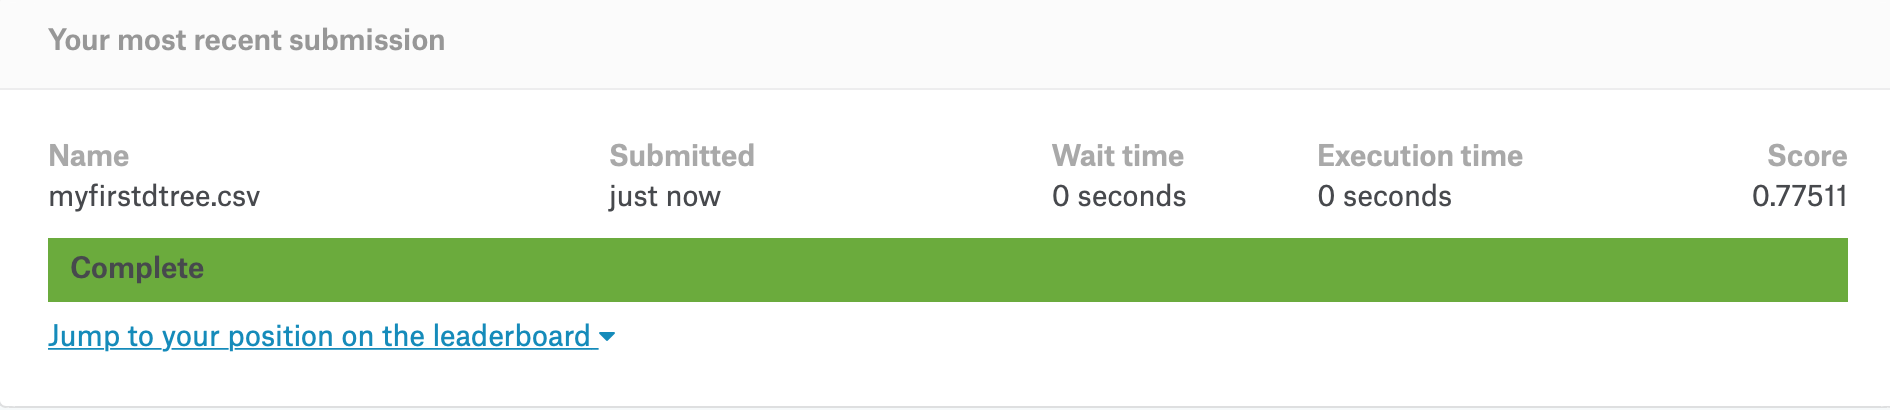
\includegraphics[width=26.25in]{Submission5}

\end{frame}

\begin{frame}[fragile]{Об'єднаємо вибірки}
\protect\hypertarget{ux43eux431ux454ux434ux43dux430ux454ux43cux43e-ux432ux438ux431ux456ux440ux43aux438}{}

\begin{Shaded}
\begin{Highlighting}[]
\NormalTok{train}\OperatorTok{$}\NormalTok{Fare2 <-}\StringTok{ }\OtherTok{NULL}
\NormalTok{train}\OperatorTok{$}\NormalTok{FamilySize <-}\StringTok{ }\OtherTok{NULL}
\NormalTok{combi <-}\StringTok{ }\KeywordTok{rbind}\NormalTok{(train, test)}
\end{Highlighting}
\end{Shaded}

\end{frame}

\begin{frame}[fragile]{}
\protect\hypertarget{section}{}

\begin{Shaded}
\begin{Highlighting}[]
\NormalTok{combi}\OperatorTok{$}\NormalTok{Title <-}\StringTok{ }\KeywordTok{gsub}\NormalTok{(}\StringTok{"^.*, (.*?)}\CharTok{\textbackslash{}\textbackslash{}}\StringTok{..*$"}\NormalTok{, }\StringTok{"}\CharTok{\textbackslash{}\textbackslash{}}\StringTok{1"}\NormalTok{, combi}\OperatorTok{$}\NormalTok{Name)}
\NormalTok{combi}\OperatorTok{$}\NormalTok{Title[combi}\OperatorTok{$}\NormalTok{Title }\OperatorTok{==}\StringTok{ 'Mlle'} \OperatorTok{|}\StringTok{ }\NormalTok{combi}\OperatorTok{$}\NormalTok{Title }\OperatorTok{==}\StringTok{ 'Ms'}\NormalTok{] <-}\StringTok{ 'Miss'} 
\NormalTok{combi}\OperatorTok{$}\NormalTok{Title[combi}\OperatorTok{$}\NormalTok{Title }\OperatorTok{==}\StringTok{ 'Mme'}\NormalTok{]  <-}\StringTok{ 'Mrs'} 
\NormalTok{combi}\OperatorTok{$}\NormalTok{Title[combi}\OperatorTok{$}\NormalTok{Title }\OperatorTok\StringTok{ }\KeywordTok{c}\NormalTok{(}\StringTok{'Capt'}\NormalTok{, }\StringTok{'Don'}\NormalTok{, }\StringTok{'Major'}\NormalTok{, }\StringTok{'Sir'}\NormalTok{, }\StringTok{'Jonkheer'}\NormalTok{)] <-}\StringTok{ 'Sir'}
\NormalTok{combi}\OperatorTok{$}\NormalTok{Title[combi}\OperatorTok{$}\NormalTok{Title }\OperatorTok\StringTok{ }\KeywordTok{c}\NormalTok{(}\StringTok{'Dona'}\NormalTok{, }\StringTok{'Lady'}\NormalTok{, }\StringTok{'the Countess'}\NormalTok{)] <-}\StringTok{ 'Lady'}
\KeywordTok{table}\NormalTok{(combi}\OperatorTok{$}\NormalTok{Title)}
\end{Highlighting}
\end{Shaded}

\begin{verbatim}
## 
##    Col     Dr   Lady Master   Miss     Mr    Mrs    Rev    Sir 
##      4      8      3     61    264    757    198      8      6
\end{verbatim}

\end{frame}

\begin{frame}[fragile]{}
\protect\hypertarget{section-1}{}

\begin{Shaded}
\begin{Highlighting}[]
\NormalTok{combi}\OperatorTok{$}\NormalTok{FamilySize <-}\StringTok{ }\NormalTok{combi}\OperatorTok{$}\NormalTok{SibSp }\OperatorTok{+}\StringTok{ }\NormalTok{combi}\OperatorTok{$}\NormalTok{Parch }\OperatorTok{+}\StringTok{ }\DecValTok{1}
\NormalTok{combi}\OperatorTok{$}\NormalTok{Surname <-}\StringTok{ }\KeywordTok{sapply}\NormalTok{(combi}\OperatorTok{$}\NormalTok{Name, }\DataTypeTok{FUN=}\ControlFlowTok{function}\NormalTok{(x) \{}\KeywordTok{strsplit}\NormalTok{(x, }\DataTypeTok{split=}\StringTok{'[,.]'}\NormalTok{)[[}\DecValTok{1}\NormalTok{]][}\DecValTok{1}\NormalTok{]\})}
\NormalTok{combi}\OperatorTok{$}\NormalTok{FamilyID <-}\StringTok{ }\KeywordTok{paste}\NormalTok{(}\KeywordTok{as.character}\NormalTok{(combi}\OperatorTok{$}\NormalTok{FamilySize), combi}\OperatorTok{$}\NormalTok{Surname, }\DataTypeTok{sep=}\StringTok{""}\NormalTok{)}
\NormalTok{combi}\OperatorTok{$}\NormalTok{FamilyID[combi}\OperatorTok{$}\NormalTok{FamilySize }\OperatorTok{<=}\StringTok{ }\DecValTok{2}\NormalTok{] <-}\StringTok{ 'Small'}
\KeywordTok{table}\NormalTok{(combi}\OperatorTok{$}\NormalTok{FamilyID)}
\end{Highlighting}
\end{Shaded}

\begin{verbatim}
## 
##            11Sage           3Abbott         3Appleton         3Beckwith 
##                11                 3                 1                 2 
##           3Boulos           3Bourke            3Brown         3Caldwell 
##                 3                 3                 4                 3 
##          3Christy          3Collyer          3Compton          3Cornell 
##                 2                 3                 3                 1 
##           3Coutts           3Crosby           3Danbom           3Davies 
##                 3                 3                 3                 5 
##            3Dodge          3Douglas             3Drew            3Elias 
##                 3                 1                 3                 3 
##       3Frauenthal        3Frolicher 3Frolicher-Stehli        3Goldsmith 
##                 1                 1                 2                 3 
##       3Gustafsson       3Hamalainen           3Hansen             3Hart 
##                 2                 2                 1                 3 
##             3Hays          3Hickman         3Hiltunen         3Hirvonen 
##                 2                 3                 1                 1 
##         3Jefferys          3Johnson             3Kink    3Kink-Heilmann 
##                 2                 3                 2                 2 
##           3Klasen         3Lahtinen           3Mallet            3McCoy 
##                 3                 2                 3                 3 
##          3Minahan         3Moubarek            3Nakid         3Navratil 
##                 1                 3                 3                 3 
##           3Newell           3Newsom         3Nicholls          3Peacock 
##                 1                 1                 1                 3 
##            3Peter            3Quick         3Richards          3Rosblom 
##                 3                 3                 2                 3 
##           3Samaan        3Sandstrom           3Silven          3Spedden 
##                 3                 3                 1                 3 
##            3Strom          3Taussig           3Thayer           3Thomas 
##                 1                 3                 3                 1 
##            3Touma     3van Billiard         3Van Impe    3Vander Planke 
##                 3                 3                 3                 2 
##            3Wells             3Wick          3Widener          4Allison 
##                 3                 3                 3                 4 
##        4Backstrom          4Baclini           4Becker           4Carter 
##                 1                 4                 4                 4 
##         4Davidson             4Dean           4Herman          4Hocking 
##                 1                 4                 4                 2 
##        4Jacobsohn         4Johnston          4Laroche           4Renouf 
##                 1                 4                 4                 1 
##    4Vander Planke             4West             5Ford          5Hocking 
##                 1                 4                 5                 1 
##    5Kink-Heilmann          5Lefebre          5Palsson          5Ryerson 
##                 1                 5                 5                 5 
##          6Fortune           6Panula             6Rice         6Richards 
##                 6                 6                 6                 1 
##            6Skoog        7Andersson          7Asplund          8Goodwin 
##                 6                 9                 7                 8 
##             Small 
##              1025
\end{verbatim}

\end{frame}

\begin{frame}[fragile]{Потрібно очистити некоректні прізвища}
\protect\hypertarget{ux43fux43eux442ux440ux456ux431ux43dux43e-ux43eux447ux438ux441ux442ux438ux442ux438-ux43dux435ux43aux43eux440ux435ux43aux442ux43dux456-ux43fux440ux456ux437ux432ux438ux449ux430}{}

\begin{Shaded}
\begin{Highlighting}[]
\NormalTok{famIDs <-}\StringTok{ }\KeywordTok{data.frame}\NormalTok{(}\KeywordTok{table}\NormalTok{(combi}\OperatorTok{$}\NormalTok{FamilyID))}
\NormalTok{famIDs <-}\StringTok{ }\NormalTok{famIDs[famIDs}\OperatorTok{$}\NormalTok{Freq }\OperatorTok{<=}\StringTok{ }\DecValTok{2}\NormalTok{,]}
\NormalTok{famIDs}
\end{Highlighting}
\end{Shaded}

\begin{verbatim}
##                 Var1 Freq
## 3          3Appleton    1
## 4          3Beckwith    2
## 9           3Christy    2
## 12          3Cornell    1
## 18          3Douglas    1
## 21       3Frauenthal    1
## 22        3Frolicher    1
## 23 3Frolicher-Stehli    2
## 25       3Gustafsson    2
## 26       3Hamalainen    2
## 27           3Hansen    1
## 29             3Hays    2
## 31         3Hiltunen    1
## 32         3Hirvonen    1
## 33         3Jefferys    2
## 35             3Kink    2
## 36    3Kink-Heilmann    2
## 38         3Lahtinen    2
## 41          3Minahan    1
## 45           3Newell    1
## 46           3Newsom    1
## 47         3Nicholls    1
## 51         3Richards    2
## 55           3Silven    1
## 57            3Strom    1
## 60           3Thomas    1
## 64    3Vander Planke    2
## 69        4Backstrom    1
## 73         4Davidson    1
## 76          4Hocking    2
## 77        4Jacobsohn    1
## 80           4Renouf    1
## 81    4Vander Planke    1
## 84          5Hocking    1
## 85    5Kink-Heilmann    1
## 92         6Richards    1
\end{verbatim}

\end{frame}

\begin{frame}[fragile]{Видалимо маленькі сім}
\protect\hypertarget{ux432ux438ux434ux430ux43bux438ux43cux43e-ux43cux430ux43bux435ux43dux44cux43aux456-ux441ux456ux43c}{}

\begin{Shaded}
\begin{Highlighting}[]
\NormalTok{combi}\OperatorTok{$}\NormalTok{FamilyID[combi}\OperatorTok{$}\NormalTok{FamilyID }\OperatorTok\StringTok{ }\NormalTok{famIDs}\OperatorTok{$}\NormalTok{Var1] <-}\StringTok{ 'Small'}
\NormalTok{combi}\OperatorTok{$}\NormalTok{FamilyID <-}\StringTok{ }\KeywordTok{factor}\NormalTok{(combi}\OperatorTok{$}\NormalTok{FamilyID)}
\end{Highlighting}
\end{Shaded}

\end{frame}

\begin{frame}[fragile]{Розділимо датасети}
\protect\hypertarget{ux440ux43eux437ux434ux456ux43bux438ux43cux43e-ux434ux430ux442ux430ux441ux435ux442ux438}{}

\begin{Shaded}
\begin{Highlighting}[]
\NormalTok{train <-}\StringTok{ }\NormalTok{combi[}\DecValTok{1}\OperatorTok{:}\DecValTok{891}\NormalTok{,]}
\NormalTok{test <-}\StringTok{ }\NormalTok{combi[}\DecValTok{892}\OperatorTok{:}\DecValTok{1309}\NormalTok{,]}
\end{Highlighting}
\end{Shaded}

\end{frame}

\begin{frame}[fragile]{Дерево нове}
\protect\hypertarget{ux434ux435ux440ux435ux432ux43e-ux43dux43eux432ux435}{}

\begin{Shaded}
\begin{Highlighting}[]
\NormalTok{fit <-}\StringTok{ }\KeywordTok{rpart}\NormalTok{(Survived }\OperatorTok{~}\StringTok{ }\NormalTok{Pclass }\OperatorTok{+}\StringTok{ }\NormalTok{Sex }\OperatorTok{+}\StringTok{ }\NormalTok{Age }\OperatorTok{+}\StringTok{ }\NormalTok{SibSp }\OperatorTok{+}\StringTok{ }\NormalTok{Parch }\OperatorTok{+}\StringTok{ }\NormalTok{Fare }\OperatorTok{+}\StringTok{ }\NormalTok{Embarked }\OperatorTok{+}\StringTok{ }\NormalTok{Title }\OperatorTok{+}\StringTok{ }\NormalTok{FamilySize }\OperatorTok{+}\StringTok{ }\NormalTok{FamilyID,}
               \DataTypeTok{data=}\NormalTok{train, }
               \DataTypeTok{method=}\StringTok{"class"}\NormalTok{)}
\KeywordTok{fancyRpartPlot}\NormalTok{(fit)}
\end{Highlighting}
\end{Shaded}

\includegraphics{Lecture8_files/figure-beamer/unnamed-chunk-48-1.pdf}

\end{frame}

\begin{frame}[fragile]{Є покращення для дерева, але гірше за нашу просту
модель}
\protect\hypertarget{ux454-ux43fux43eux43aux440ux430ux449ux435ux43dux43dux44f-ux434ux43bux44f-ux434ux435ux440ux435ux432ux430-ux430ux43bux435-ux433ux456ux440ux448ux435-ux437ux430-ux43dux430ux448ux443-ux43fux440ux43eux441ux442ux443-ux43cux43eux434ux435ux43bux44c-1}{}

\begin{Shaded}
\begin{Highlighting}[]
\NormalTok{Prediction <-}\StringTok{ }\KeywordTok{predict}\NormalTok{(fit, test, }\DataTypeTok{type =} \StringTok{"class"}\NormalTok{)}
\NormalTok{submit <-}\StringTok{ }\KeywordTok{data.frame}\NormalTok{(}\DataTypeTok{PassengerId =}\NormalTok{ test}\OperatorTok{$}\NormalTok{PassengerId, }\DataTypeTok{Survived =}\NormalTok{ Prediction)}
\KeywordTok{write.csv}\NormalTok{(submit, }\DataTypeTok{file =} \StringTok{"myfirstdtree.csv"}\NormalTok{, }\DataTypeTok{row.names =} \OtherTok{FALSE}\NormalTok{)}
\end{Highlighting}
\end{Shaded}

\end{frame}

\begin{frame}[fragile]{Так, ми покращили результат!}
\protect\hypertarget{ux442ux430ux43a-ux43cux438-ux43fux43eux43aux440ux430ux449ux438ux43bux438-ux440ux435ux437ux443ux43bux44cux442ux430ux442}{}

\begin{Shaded}
\begin{Highlighting}[]
\NormalTok{knitr}\OperatorTok{::}\KeywordTok{include_graphics}\NormalTok{(}\StringTok{"Submission6.png"}\NormalTok{)}
\end{Highlighting}
\end{Shaded}


\includegraphics[width=26.75in]{Submission6}

\end{frame}

\begin{frame}[fragile]{Випадкові ліси. Модифікуємо склад сім'ї}
\protect\hypertarget{ux432ux438ux43fux430ux434ux43aux43eux432ux456-ux43bux456ux441ux438.-ux43cux43eux434ux438ux444ux456ux43aux443ux454ux43cux43e-ux441ux43aux43bux430ux434-ux441ux456ux43cux457}{}

\begin{Shaded}
\begin{Highlighting}[]
\NormalTok{combi}\OperatorTok{$}\NormalTok{FamilyID2 <-}\StringTok{ }\NormalTok{combi}\OperatorTok{$}\NormalTok{FamilyID}
\NormalTok{combi}\OperatorTok{$}\NormalTok{FamilyID2 <-}\StringTok{ }\KeywordTok{as.character}\NormalTok{(combi}\OperatorTok{$}\NormalTok{FamilyID2)}
\NormalTok{combi}\OperatorTok{$}\NormalTok{FamilyID2[combi}\OperatorTok{$}\NormalTok{FamilySize }\OperatorTok{<=}\StringTok{ }\DecValTok{3}\NormalTok{] <-}\StringTok{ 'Small'}
\NormalTok{combi}\OperatorTok{$}\NormalTok{FamilyID2 <-}\StringTok{ }\KeywordTok{factor}\NormalTok{(combi}\OperatorTok{$}\NormalTok{FamilyID2)}

\NormalTok{combi}\OperatorTok{$}\NormalTok{Title <-}\StringTok{ }\KeywordTok{factor}\NormalTok{(combi}\OperatorTok{$}\NormalTok{Title)}

\NormalTok{combi}\OperatorTok{$}\NormalTok{Fare2 <-}\StringTok{ '30+'}
\NormalTok{combi}\OperatorTok{$}\NormalTok{Fare2[combi}\OperatorTok{$}\NormalTok{Fare }\OperatorTok{<}\StringTok{ }\DecValTok{30} \OperatorTok{&}\StringTok{ }\NormalTok{combi}\OperatorTok{$}\NormalTok{Fare }\OperatorTok{>=}\StringTok{ }\DecValTok{20}\NormalTok{] <-}\StringTok{ '20-30'}
\NormalTok{combi}\OperatorTok{$}\NormalTok{Fare2[combi}\OperatorTok{$}\NormalTok{Fare }\OperatorTok{<}\StringTok{ }\DecValTok{20} \OperatorTok{&}\StringTok{ }\NormalTok{combi}\OperatorTok{$}\NormalTok{Fare }\OperatorTok{>=}\StringTok{ }\DecValTok{10}\NormalTok{] <-}\StringTok{ '10-20'}
\NormalTok{combi}\OperatorTok{$}\NormalTok{Fare2[combi}\OperatorTok{$}\NormalTok{Fare }\OperatorTok{<}\StringTok{ }\DecValTok{10}\NormalTok{] <-}\StringTok{ '<10'}
\NormalTok{combi}\OperatorTok{$}\NormalTok{Fare2 <-}\StringTok{ }\KeywordTok{factor}\NormalTok{(combi}\OperatorTok{$}\NormalTok{Fare2)}
\end{Highlighting}
\end{Shaded}

\end{frame}

\begin{frame}[fragile]{Додаємо ліси}
\protect\hypertarget{ux434ux43eux434ux430ux454ux43cux43e-ux43bux456ux441ux438}{}

\begin{Shaded}
\begin{Highlighting}[]
\KeywordTok{library}\NormalTok{(randomForest)}
\end{Highlighting}
\end{Shaded}

\begin{verbatim}
## randomForest 4.6-14
\end{verbatim}

\begin{verbatim}
## Type rfNews() to see new features/changes/bug fixes.
\end{verbatim}

\begin{verbatim}
## 
## Attaching package: 'randomForest'
\end{verbatim}

\begin{verbatim}
## The following object is masked from 'package:rattle':
## 
##     importance
\end{verbatim}

\begin{verbatim}
## The following object is masked from 'package:dplyr':
## 
##     combine
\end{verbatim}

\begin{verbatim}
## The following object is masked from 'package:ggplot2':
## 
##     margin
\end{verbatim}

\begin{Shaded}
\begin{Highlighting}[]
\KeywordTok{set.seed}\NormalTok{(}\DecValTok{415}\NormalTok{)}
\end{Highlighting}
\end{Shaded}

\end{frame}

\begin{frame}[fragile]{Запустити просто}
\protect\hypertarget{ux437ux430ux43fux443ux441ux442ux438ux442ux438-ux43fux440ux43eux441ux442ux43e}{}

\begin{Shaded}
\begin{Highlighting}[]
\NormalTok{train <-}\StringTok{ }\NormalTok{combi[}\DecValTok{1}\OperatorTok{:}\DecValTok{891}\NormalTok{,]}
\NormalTok{test <-}\StringTok{ }\NormalTok{combi[}\DecValTok{892}\OperatorTok{:}\DecValTok{1309}\NormalTok{,]}
\KeywordTok{colSums}\NormalTok{(}\KeywordTok{is.na}\NormalTok{(train)}\OperatorTok{|}\NormalTok{train}\OperatorTok{==}\StringTok{''}\NormalTok{)}
\end{Highlighting}
\end{Shaded}

\begin{verbatim}
## PassengerId    Survived      Pclass        Name         Sex         Age 
##           0           0           0           0           0           0 
##       SibSp       Parch      Ticket        Fare       Cabin    Embarked 
##           0           0           0           0         687           0 
##       Child       Title  FamilySize     Surname    FamilyID   FamilyID2 
##           0           0           0           0           0           0 
##       Fare2 
##           0
\end{verbatim}

\begin{Shaded}
\begin{Highlighting}[]
\NormalTok{fit <-}\StringTok{ }\KeywordTok{randomForest}\NormalTok{(}\KeywordTok{as.factor}\NormalTok{(Survived) }\OperatorTok{~}\StringTok{ }\NormalTok{Pclass }\OperatorTok{+}\StringTok{ }\NormalTok{Sex }\OperatorTok{+}\StringTok{ }\NormalTok{Age  }\OperatorTok{+}\StringTok{ }\NormalTok{Fare2 }\OperatorTok{+}
\StringTok{                                            }\NormalTok{Embarked }\OperatorTok{+}\StringTok{ }\NormalTok{Title }\OperatorTok{+}\StringTok{ }\NormalTok{FamilySize }\OperatorTok{+}\StringTok{ }\NormalTok{FamilyID2,}
                      \DataTypeTok{data=}\NormalTok{train, }
                      \DataTypeTok{importance=}\OtherTok{TRUE}\NormalTok{, }
                      \DataTypeTok{ntree=}\DecValTok{2000}\NormalTok{)}
\end{Highlighting}
\end{Shaded}

\end{frame}

\begin{frame}[fragile]{Що там в середині}
\protect\hypertarget{ux449ux43e-ux442ux430ux43c-ux432-ux441ux435ux440ux435ux434ux438ux43dux456}{}

\begin{Shaded}
\begin{Highlighting}[]
\KeywordTok{varImpPlot}\NormalTok{(fit)}
\end{Highlighting}
\end{Shaded}

\includegraphics{Lecture8_files/figure-beamer/unnamed-chunk-54-1.pdf}

\end{frame}

\begin{frame}[fragile]{Створюємо передбачення}
\protect\hypertarget{ux441ux442ux432ux43eux440ux44eux454ux43cux43e-ux43fux435ux440ux435ux434ux431ux430ux447ux435ux43dux43dux44f}{}

\begin{Shaded}
\begin{Highlighting}[]
\NormalTok{Prediction <-}\StringTok{ }\KeywordTok{predict}\NormalTok{(fit, test)}
\NormalTok{submit <-}\StringTok{ }\KeywordTok{data.frame}\NormalTok{(}\DataTypeTok{PassengerId =}\NormalTok{ test}\OperatorTok{$}\NormalTok{PassengerId, }\DataTypeTok{Survived =}\NormalTok{ Prediction)}
\KeywordTok{write.csv}\NormalTok{(submit, }\DataTypeTok{file =} \StringTok{"firstforest.csv"}\NormalTok{, }\DataTypeTok{row.names =} \OtherTok{FALSE}\NormalTok{)}
\end{Highlighting}
\end{Shaded}

\end{frame}

\begin{frame}[fragile]{}
\protect\hypertarget{section-2}{}

\begin{Shaded}
\begin{Highlighting}[]
\KeywordTok{library}\NormalTok{(party)}
\end{Highlighting}
\end{Shaded}

\begin{verbatim}
## Loading required package: grid
\end{verbatim}

\begin{verbatim}
## Loading required package: mvtnorm
\end{verbatim}

\begin{verbatim}
## Loading required package: modeltools
\end{verbatim}

\begin{verbatim}
## Loading required package: stats4
\end{verbatim}

\begin{verbatim}
## Loading required package: strucchange
\end{verbatim}

\begin{verbatim}
## Loading required package: zoo
\end{verbatim}

\begin{verbatim}
## 
## Attaching package: 'zoo'
\end{verbatim}

\begin{verbatim}
## The following objects are masked from 'package:base':
## 
##     as.Date, as.Date.numeric
\end{verbatim}

\begin{verbatim}
## Loading required package: sandwich
\end{verbatim}

\begin{verbatim}
## 
## Attaching package: 'strucchange'
\end{verbatim}

\begin{verbatim}
## The following object is masked from 'package:stringr':
## 
##     boundary
\end{verbatim}

\begin{Shaded}
\begin{Highlighting}[]
\KeywordTok{set.seed}\NormalTok{(}\DecValTok{415}\NormalTok{)}
\NormalTok{fit <-}\StringTok{ }\KeywordTok{cforest}\NormalTok{(}\KeywordTok{as.factor}\NormalTok{(Survived) }\OperatorTok{~}\StringTok{ }\NormalTok{Pclass }\OperatorTok{+}\StringTok{ }\NormalTok{Sex }\OperatorTok{+}\StringTok{ }\NormalTok{Age }\OperatorTok{+}\StringTok{ }\NormalTok{SibSp }\OperatorTok{+}\StringTok{ }\NormalTok{Parch }\OperatorTok{+}\StringTok{ }\NormalTok{Fare2 }\OperatorTok{+}
\StringTok{                                       }\NormalTok{Embarked }\OperatorTok{+}\StringTok{ }\NormalTok{Title }\OperatorTok{+}\StringTok{ }\NormalTok{FamilySize }\OperatorTok{+}\StringTok{ }\NormalTok{FamilyID,}
                 \DataTypeTok{data =}\NormalTok{ train, }
                 \DataTypeTok{controls=}\KeywordTok{cforest_unbiased}\NormalTok{(}\DataTypeTok{ntree=}\DecValTok{2000}\NormalTok{, }\DataTypeTok{mtry=}\DecValTok{3}\NormalTok{))}
\end{Highlighting}
\end{Shaded}

\end{frame}

\begin{frame}[fragile]{}
\protect\hypertarget{section-3}{}

\begin{Shaded}
\begin{Highlighting}[]
\KeywordTok{set.seed}\NormalTok{(}\DecValTok{415}\NormalTok{)}
\NormalTok{fit <-}\StringTok{ }\KeywordTok{cforest}\NormalTok{(}\KeywordTok{as.factor}\NormalTok{(Survived) }\OperatorTok{~}\StringTok{ }\NormalTok{Pclass }\OperatorTok{+}\StringTok{ }\NormalTok{Sex }\OperatorTok{+}\StringTok{ }\NormalTok{Age }\OperatorTok{+}\StringTok{ }\NormalTok{SibSp }\OperatorTok{+}\StringTok{ }\NormalTok{Parch }\OperatorTok{+}\StringTok{ }\NormalTok{Fare }\OperatorTok{+}\StringTok{ }\NormalTok{Embarked }\OperatorTok{+}\StringTok{ }\NormalTok{Title }\OperatorTok{+}\StringTok{ }\NormalTok{FamilySize }\OperatorTok{+}\StringTok{ }\NormalTok{FamilyID,}
               \DataTypeTok{data =}\NormalTok{ train, }\DataTypeTok{controls=}\KeywordTok{cforest_unbiased}\NormalTok{(}\DataTypeTok{ntree=}\DecValTok{2000}\NormalTok{, }\DataTypeTok{mtry=}\DecValTok{3}\NormalTok{)) }
\CommentTok{# Now let's make a prediction and write a submission file}
\NormalTok{Prediction <-}\StringTok{ }\KeywordTok{predict}\NormalTok{(fit, test, }\DataTypeTok{OOB=}\OtherTok{TRUE}\NormalTok{, }\DataTypeTok{type =} \StringTok{"response"}\NormalTok{)}
\NormalTok{submit <-}\StringTok{ }\KeywordTok{data.frame}\NormalTok{(}\DataTypeTok{PassengerId =}\NormalTok{ test}\OperatorTok{$}\NormalTok{PassengerId, }\DataTypeTok{Survived =}\NormalTok{ Prediction)}
\KeywordTok{write.csv}\NormalTok{(submit, }\DataTypeTok{file =} \StringTok{"ciforest.csv"}\NormalTok{, }\DataTypeTok{row.names =} \OtherTok{FALSE}\NormalTok{)}
\end{Highlighting}
\end{Shaded}

\end{frame}

\end{document}
